\section{Evaluation \label{sec:evaluation}}

This section explain the divers evaluation metrics used and experiments realized on the datasets to evaluate the proposed methods (ref. Section~\ref{sec:methods}).
Each experiment of this section is described by its purpose in the study, the methodology used to conduct it, the results in the form of: graph, table or statistics, an analysis of the results and sometimes a few additional conclusion to the experiment.
The section is seperated into two parts, one concerning the rank lists and another one dedicated to the clustering task.

\subsection{Rank lists}

\subsubsection{Rank list evaluation metrics}
\label{sec:rl_eval}

In order to know the quality of a rank list, the following metrics are used.
Definitions in this sections are adapted versions of the ones in Kocher and Savoy's \textit{Evaluation of text representation schemes and distance measures for authorship linking}~\cite{kocher_linking}.
The presented metrics are well know in the authorship verification and the information retrieval field.

\begin{definition}[Relevant link~\cite{kocher_linking}]
  A relevant link is a link in the relevant set.
  The relevant set is explain in Definition~\ref{def:relevant_set}.
  \begin{equation}
    relevant(l_i) =
    \begin{cases}
      1, & if\ l_i \in R \\
      0, & otherwise
    \end{cases}
  \end{equation}
\end{definition}

\begin{definition}[Precision@k~\cite{kocher_linking}]
  The precision@k is a function which take a positive integer k, with k < |L|
  \begin{equation}
    precision(k) = \frac{1}{k} \sum_{j=1}^{k} relevant(j)
  \end{equation}
\end{definition}

\begin{definition}[Average Precision (AP)]
  The mean over the precision@k each time a relevant link is retrieved.
  \begin{equation}
    AveragePrecision = \frac{1}{|R|} \sum_{j=1}^{|L|} precision(j) \cdot relevant(j)
  \end{equation}
  The average precision can be considered as an approximation of the area under the precision-recall curve.
\end{definition}

\begin{definition}[R-Precision~\cite{kocher_linking}]
  The R-Precision (RPrec) is the precision in the rank list at rank |R| (Precision@r).
  With R being the relevant set (Definition~\ref{def:relevant_set}).
  \begin{equation}
    RPrec = precision(|R|)
  \end{equation}
  The RPrec value is in the range $\left[0, 1\right]$.
  With 0 mean every links in the first $|R|$-ranks are not in the relevant set.
  And 1, every links in the first $|R|$-ranks are in the relevant set.
\end{definition}

\begin{definition}[High precision~\cite{kocher_linking}]
  The high precision (HPrec) represent the maximal rank j in the rank list such that the precision is still 100\%.
  \begin{equation}
    HPrec = \max\{i \in \mathbf{N} | precision(i) = 1\}
  \end{equation}
  This value is in the range $\left[0, |R|\right]$.
  $0$ means the first pair in the rank list is incorrect.
  $|R|$ means every true links are ranked in the top part of the rank list.
\end{definition}

\subsubsection{Importance of the text size in stylometry}

Previous studies have shown the importance of having documents of good quality and with at least 5000 tokens to have reliable results.
Skilled authors can easily change their style to imitate others for small texts, but it becomes more difficult for larger texts~\cite{savoy_stylo}.

For this study, an experiment on the St-Jean dataset is accomplish, in the order to show the importance of having large documents.
In order to test this parameter, the number of token is artificially modified by considering only the $n$ first tokens for each text, with $n$ ranging between 9000 and 250 with steps of 250 tokens.
Figure~\ref{img:degradation} shows the three metrics used (Average precision, RPrec, HPrec) over the number of tokens.
Every metrics decrease over the text size, which indicate that it becomes harder to determinate documents pairs with the same author as the text size decrease.

\begin{figure}
  \centering
  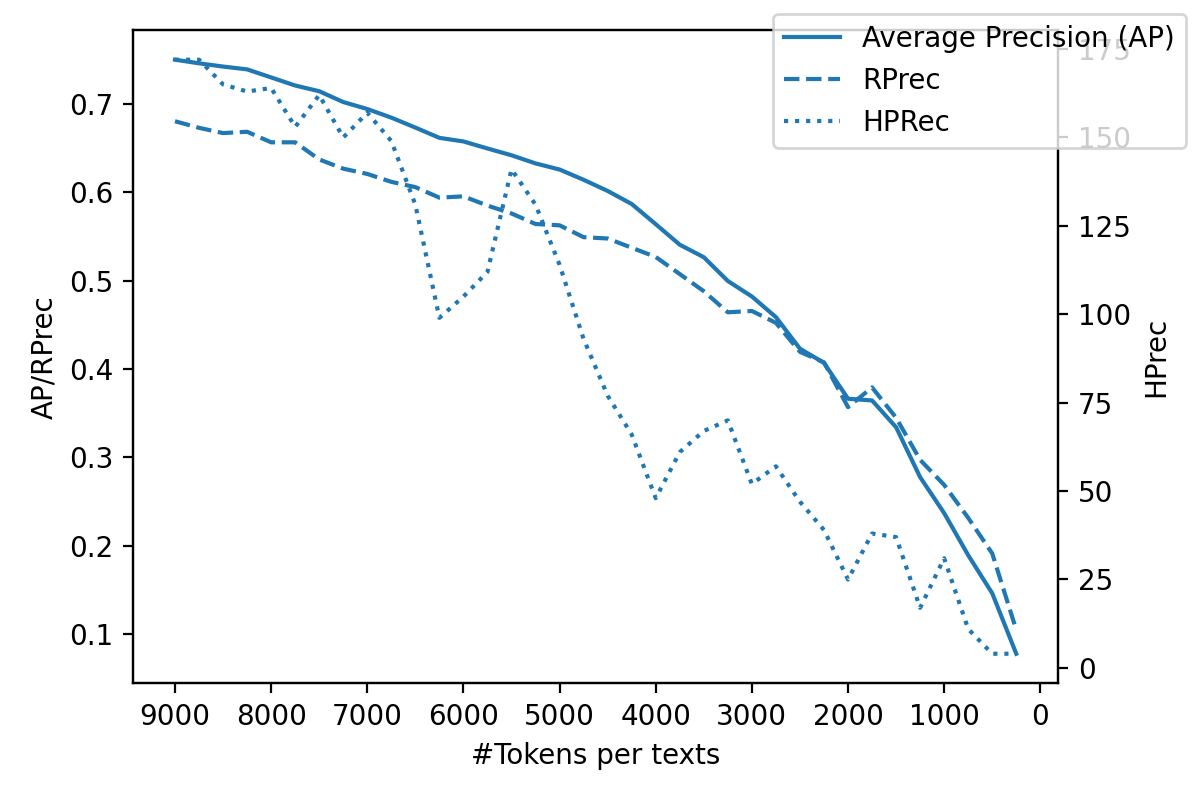
\includegraphics[width=\linewidth]{img/degradation.png}
  \caption{St-Jean ranks list evaluation on AP, RPrec and HPrec over the text size. Rank list computed using 500 MFW and the zscored-normalized cosine distance}
  \label{img:degradation}
\end{figure}

PAN16 dataset is a difficult dataset due to its small size, thus extracting reliable features for each text to estimate each style is also a difficult task.
After multiple tests, the PAN @ CLEF 2016 dataset is not used further in this study due to its difficulty in finding reliable Stylometric clues.

\subsubsection{MFW Token and Lemma}
\label{sec:mfw_token_lemma}

Here the goal is to compare two similar text representations, which are the token representation, words as they can appear in the novels, and the lemmatize representation, for example \textit{il voit} (he sees) will be lemmatized to \textit{il voir} (he see).
For this kind of representation, previous studies have shown that using MFW (most frequent words) vector size of around 500 tends to produce better outcomes~\cite{savoy_text_representation}.

After creating the rank lists with the proposed distance measures (ref. Section~\ref{sec:fv_distances}) on the two representations for a MFW vector size ranging between 100 and 2000 with a step of 100, on the two datasets containing the lemmatize representation (Brunet and St-Jean), the two plots in Figure~\ref{fig:token_vs_lemma} show the average precision (AP) for the resulting rank lists.

This representation seem to have good results with a MFW vector size of 500 for most of the metrics, this corroborate previous studies results.
A few metrics, such as Manhattan distance or Clark distance can give better results with slightly bigger vectors.
In most cases, the token representation provide on both dataset a greater average precision compared to the lemma representation.
An interesting example to be worth noticing concern the Manhattan distance, when using the token representation it tends to decrease the AP faster than the lemma representation as the MFW vector size increase.
The euclidean distance seem to be the least appropriate distance measure for this task.
The Clark distance have a really poor average precision when the MFW vector is too small but after reaching 500 it produces one of the best pay-off of the experiment.
Over all, the cosine distance seem to be one of the most appropriate choice when dealing with these datasets and text representations.
For the next experiments dealing with this text representation, four distance mesures are retained : Cosine distance, Clark, Manhattan and Tanimoto, with a MFW vector size of 750.

\begin{figure}
  \centering
  \caption{Token and Lemma representation over number of MFW using different distances metrics}
  \label{fig:token_vs_lemma}

  \subcaption{Brunet}
  \label{fig:token_vs_lemma_brunet}
  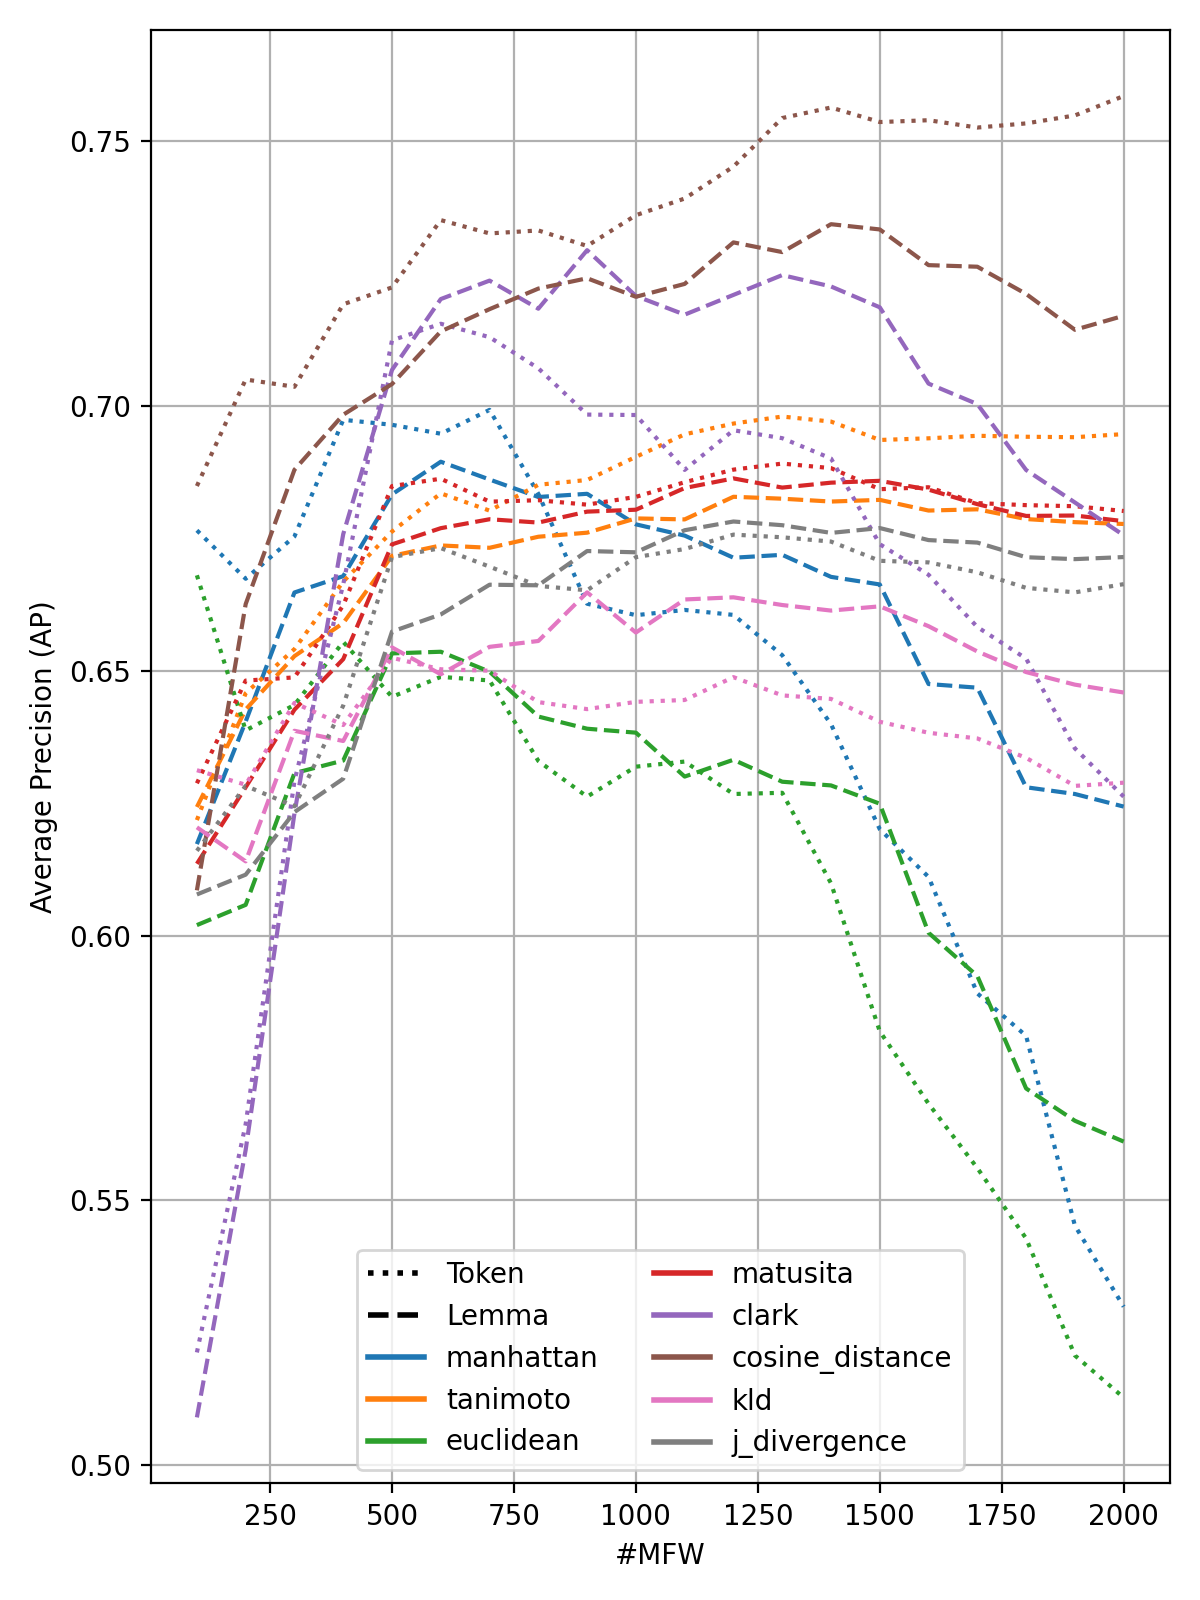
\includegraphics[width=0.9\linewidth]{img/token_vs_lemma_brunet.png}

  \subcaption{St-Jean}
  \label{fig:token_vs_lemma_st_jean}
  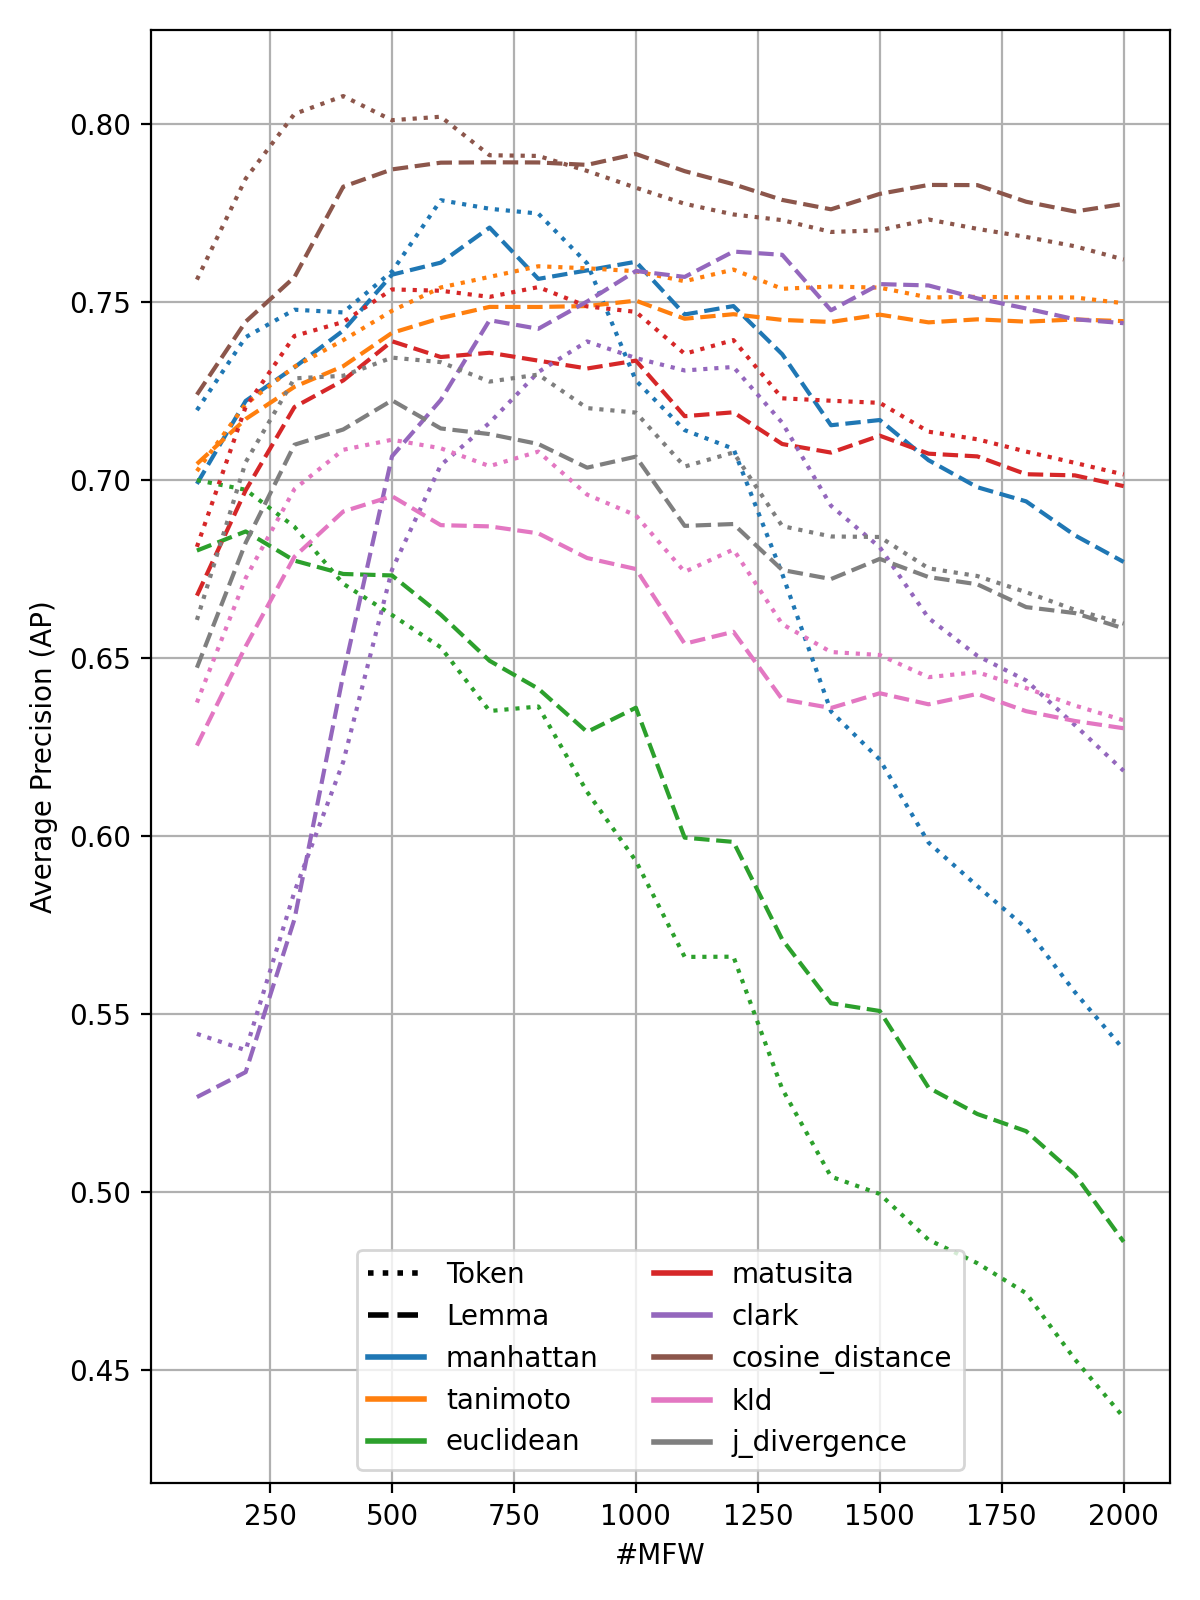
\includegraphics[width=0.9\linewidth]{img/token_vs_lemma_st_jean.png}
\end{figure}

\subsubsection{MFW Letter $n$-grams}

In this experiment the whole text is considered to create letters $n$-grams for the text representation, see Definition~\ref{def:letters_n_grams}.
As for the other experiment the MFW approach is used to create the feature vector.
On these vectors the distance measure used to create the rank list is the z-score normalized cosine distance.
The goal is to compare the influence of $n$ parameter of the $n$-grams over the size of the feature vector.
The parameters used are: a varying MFW vector size ranging between 500 and 15000 with a step of 500 and a $n$ for the following values : $3, 4, 5, (2, 3), (3, 4), (4, 5)$, the tuples $(a, b)$ correspond to both $a$-grams and $b$-grams in the same text representation.
The number of different $n$-grams is not clear, but it is assumed to be larger than the vocabulary of the texts, thus the importance of having larger vector when dealing with long texts such as the literature datasets.
When considering letters $n$-grams the text representation increase size by a factor of approximately $t$, with $t$ being the average token length.
The average token size for the literature dataset is displayed Table~\ref{tab:lit_datasets}, and is in average \~4.
To avoid having too large text representation a possible idea is to remove the hapax legomena (tokens appearing only once in the corpus) before applying the $n$-grams algorithm.
This pruning approach was explored in~\cite{kocher_linking}.

Figure~\ref{fig:letter_ngrams} show the results of this experiment on the Oxquarry dataset (\ref{fig:letter_ngrams_oxquarry}) , Brunet (\ref{fig:letter_ngrams_brunet}) and St-Jean (\ref{fig:letter_ngrams_st_jean}).
The trends seems to indicate that a lower $n$ value converge with lower MFW vector size but reach a maximal value faster.
With $3$-grams, \~3000-4000 MFW give good results on both datasets with this distance metric.
On the Brunet dataset, after reaching the maximal average precision at \~4000 MFW, a larger number of frequent words decrease the precision until reaching the maximal number of differant $3$-grams at \~6500 MFW, which is not the case on Oxquarry.
On St-Jean, the $3$-grams and $(2,3)$-grams don't reach high average precision on low number of MFW like for the Brunet and Oxquarry.
$4$-grams also can be efficient but require a larger MFW vector, around \~4000 good result for both Brunet and St-Jean but on Oxquarry it requires around \~8000 to have similar results as the 3000 $3$-grams.
Even though other distance metrics can give different results,
For the letters $n$-grams text representation, the retained configurations for next experiments are : $3$-grams with 3000 MFWs and $4$-grams with 8000 MFWs.

\begin{figure}
  \caption{Letters $n$-grams representation over number of MFW with different $n$}
  \label{fig:letter_ngrams}

  \subcaption{Oxquarry}
  \label{fig:letter_ngrams_oxquarry}
  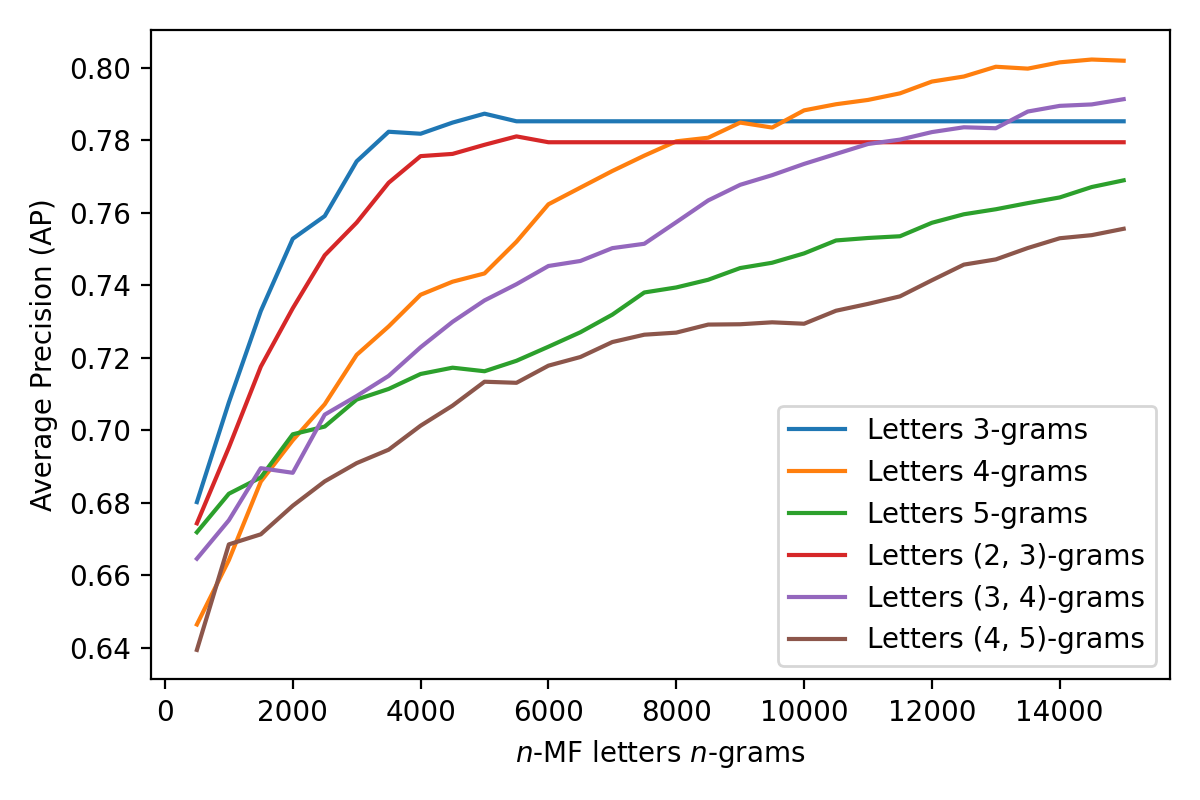
\includegraphics[width=\linewidth]{img/letter_ngrams_oxquarry.png}

  \subcaption{Brunet}
  \label{fig:letter_ngrams_brunet}
  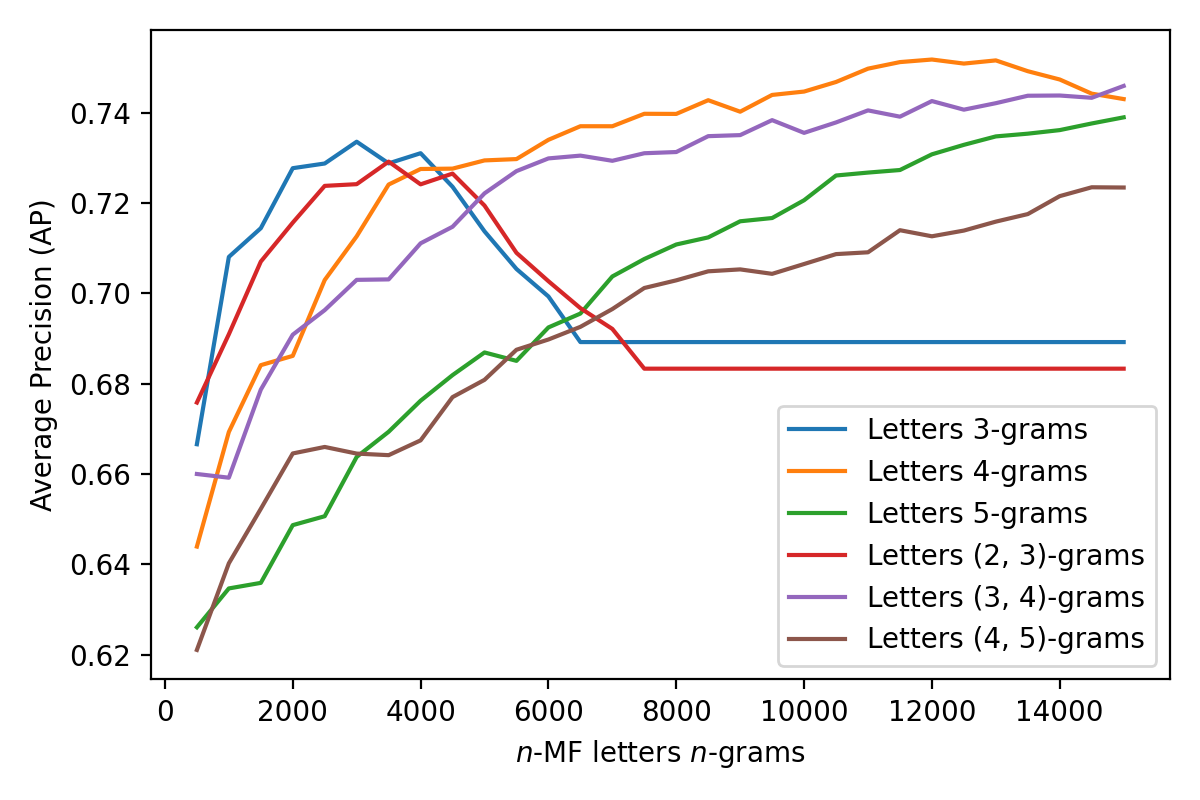
\includegraphics[width=\linewidth]{img/letter_ngrams_brunet.png}

  \subcaption{St-Jean}
  \label{fig:letter_ngrams_st_jean}
  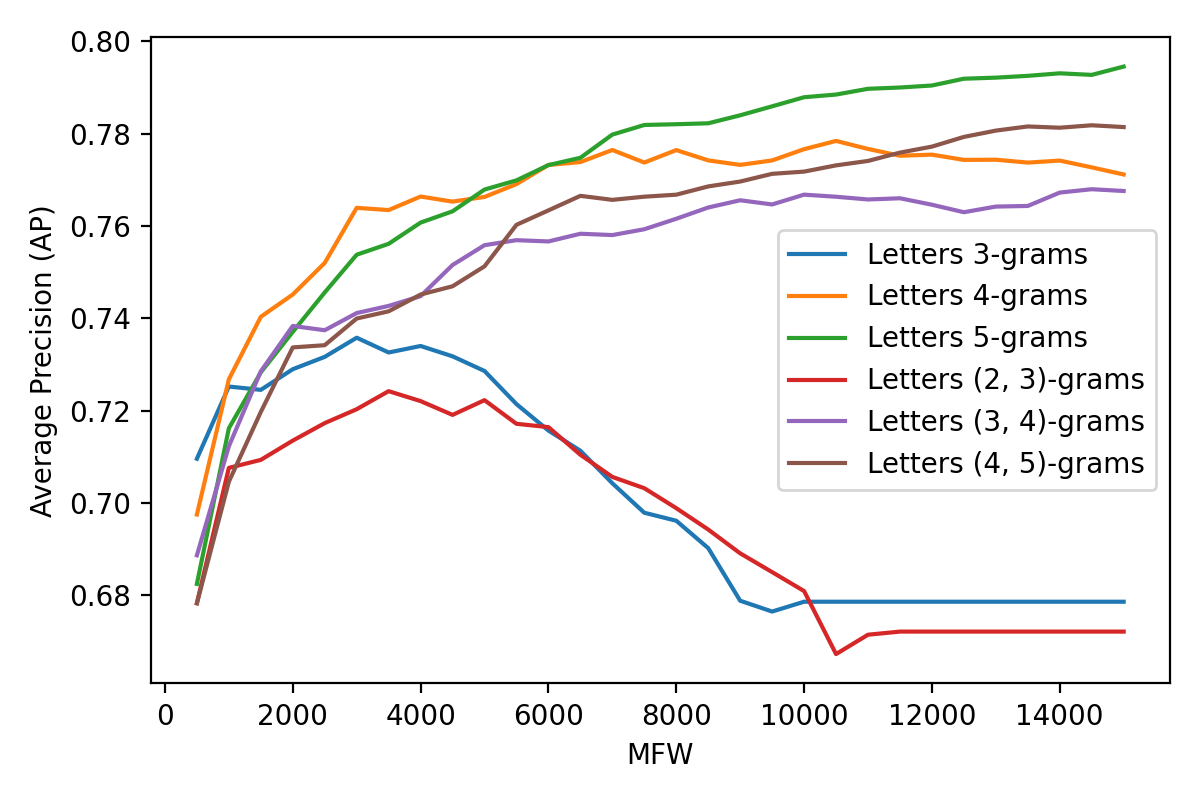
\includegraphics[width=\linewidth]{img/letter_ngrams_st_jean.png}
\end{figure}

\subsubsection{MFW First letters, last letters, word n-grams of tokens}

In this experiment, the goal is to create 3 types of text representations of word substrings and compare them.

\begin{enumerate}
  \item
  The first representation is the N-first letter of each word tokens which correspond generaly to the meaning of a word.
  If the word token is smaller than N, the whole word is used.
  This approach can be related to the lemma approach.
  \item
  Extract also the N-last letter of each word tokens which in this case correspond to the role of the word in a sentence.
  As for the previous representation, if the word is smaller than N, the whole is used instead.
  This second approach can be related to the POS approach.
  \item
  The in-word $n$-grams (See Definition~\ref{def:words_n_grams}), this special type of n-grams consider only $n$-grams within a word.
  This exclude every overlapping word when considering the Letters $n$-grams algorithm.
  This decision is made for this experiment such that interwords style information can't be learned and have a fair comparaison of these 3 texts representations.
\end{enumerate}
The third method can be considered as a hybride version between the letters $n$-grams and the word token text representations.
This representation is also smaller then the Letters $n$-grams text representation.
The two first representation are subsets of the thrid method.

For this experiment the only distance measure used is the z-normalized cosine distance and, for the evaluation metric only the average precision.
The number of MFW variate for this experiment between 200 and 4000 with a step of 100.

Figure~\ref{fig:first_last_letters_ngrams_brunet} shows the results for the Brunet dataset and Figure~\ref{fig:first_last_letters_ngrams_oxquarry} for the oxquarry dataset.

In both dataset, the 3-last letters and 3-first letters gives a lower average precision and quickly converge to a equilibrium value at around 1500 MFW.
5-letters representations tend to produce better results than 3-letters and 4-letters representation as the MFW increase.
In the Oxquarry corpus, word 4-grams and word 5-grams give the better results with an average precision of ~95.0\%.
For the Brunet dataset, the 5-first letters can a good results compared to other text representations with small MFW vector size.

\begin{figure}
  \centering
  \caption{Average precision over the MFW in the rank list generated using the z-score normalized cosine distance}

  \subcaption{Oxquarry}
  \label{fig:first_last_letters_ngrams_oxquarry}
  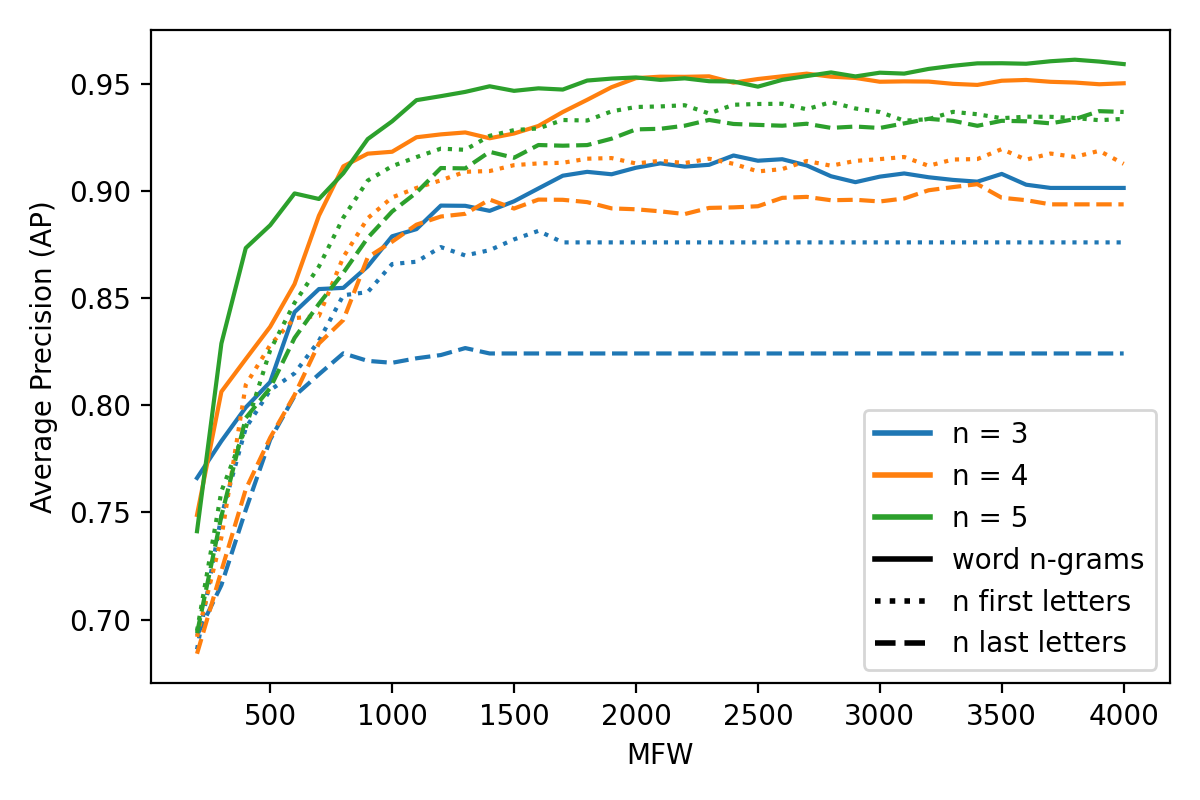
\includegraphics[width=\linewidth]{img/first_last_letters_ngrams_oxquarry.png}

  \subcaption{Brunet}
  \label{fig:first_last_letters_ngrams_brunet}
  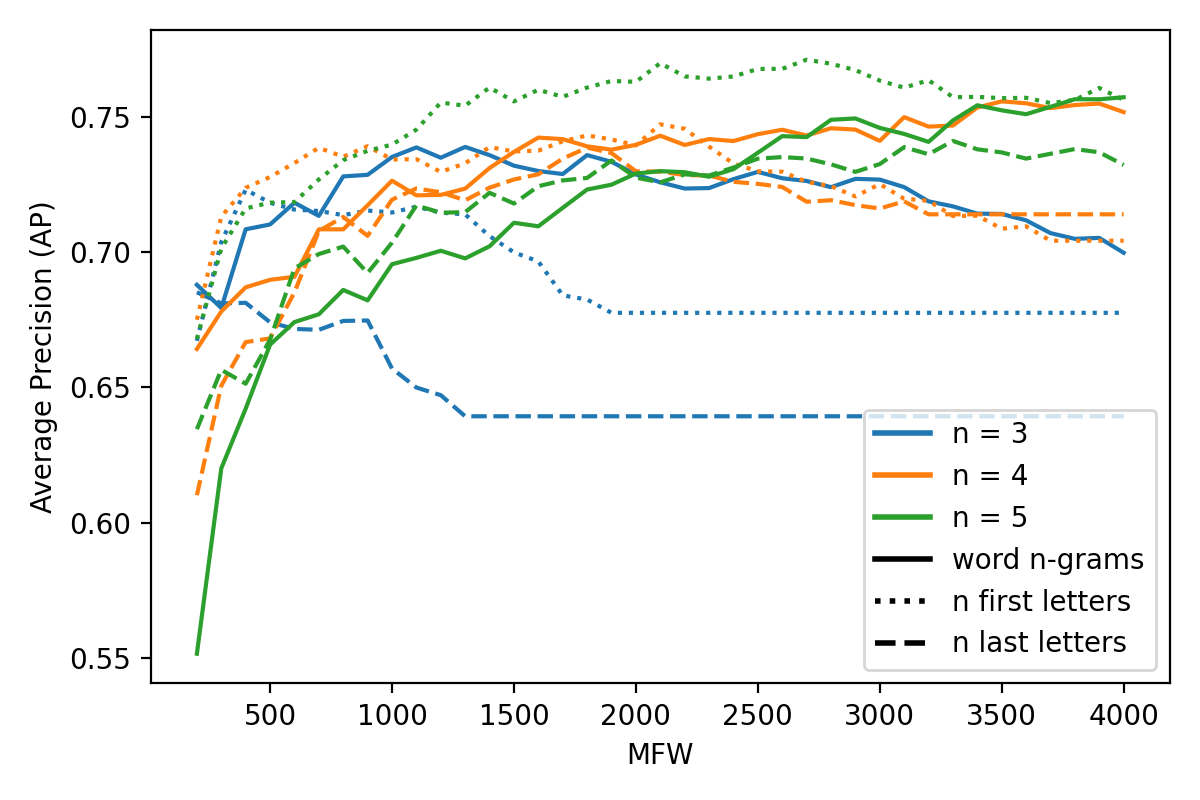
\includegraphics[width=\linewidth]{img/first_last_letters_ngrams_brunet.png}
\end{figure}

\subsubsection{MFW POS $n$-grams}

For this experiment short combination of POS are used to detect the style of the author.
The St-Jean dataset have for every word a POS tag, by using these POS tags and combining them using Definition~\ref{def:letters_n_grams} to create $n$-grams/w-shingling, a new text representation is obtained.
Using this representation the N-MFW are computed and the rank list containing every document pairs can be computed.

In this experiment, only $2$-grams, $3$-grams, $4$-grams and the combination of the $2$-grams and $3$-grams denoted: $(2, 3)$-grams is used.
The distance metric used is the smoothed z-score normalized cosine distance.
For this representation no clear MFW (most frequent word, in this case POS $n$-grams are considered as words) vector size is advised, the size used is between 200 and 2000 with a step of 100.
Figure~\ref{fig:pos_ngrams} show the average precision on the rank list produced by using POS $n$-grams over the number of MFW.

The two following informations can be intuitively observed on this plot:
\begin{itemize}
  \item
  A more complex POS $n$-grams require more MFW to archive its maximal effectiveness.
  In the St-Jean corpus, 26 POS are used to describe every words in the corpus.
  Which correspond to $26^2 = 676$ possible unique POS $2$-grams, to $26^3 = 17'576$ POS $3$-grams and $26^4 = 456'976$ POS $4$-grams, thus the the convergence of $2$-grams and not $3$-grams / $4$-grams.
  \item
  Like other methods, if the MFW ceiling is too high, an overfitting to less important words is possible, thus reducing the average precision.
  In Figure~\ref{fig:pos_ngrams} the POS 2-grams clearly have a drop in average precision after \~250-MFW.
\end{itemize}

The most appropriate configuration for the POS $n$-grams text representation on St-Jean seem to be 250 MFW POS $2$-grams and 1000 MFW POS $3$-grams.

\begin{figure}
  \centering
  \caption{Average precision over the MFW in the rank list generated using the z-score normalized cosine distance on St-Jean POS n-grams text representation.}
  \label{fig:pos_ngrams}
  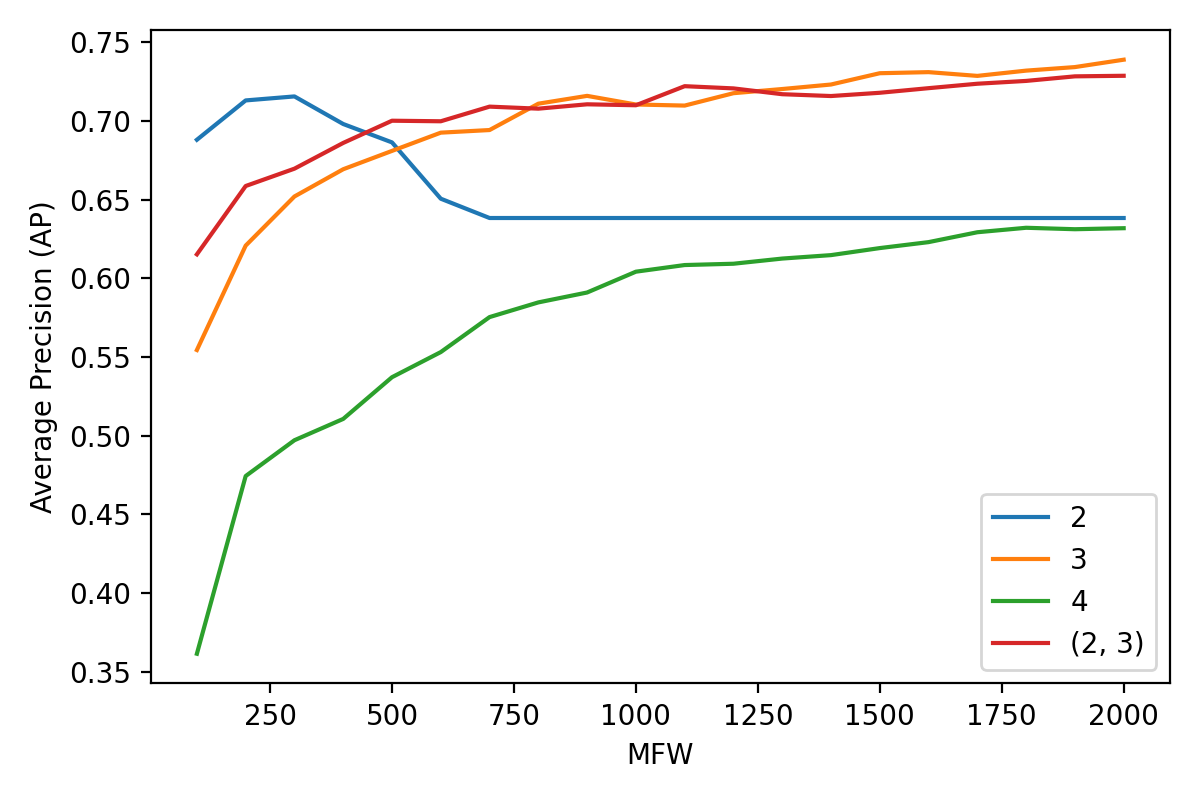
\includegraphics[width=\linewidth]{img/pos_ngrams.png}
\end{figure}

\subsubsection{Compression based distances}

This experiment try to compare the three proposed compression algorithm (GZip, BZip2, LZMA) for the compression based distance ranking.
For each algorithm and for each document, the size after compression is computed, as well as the concatenation of every document pairs.
Using these sizes and the NCD and CBC distance metrics (ref. Section~\ref{sec:compression_based_distances}, the rank list is evaluated.
This experiment is run on the three datasets three times to have a better approximation of the run time.
The results in terms of efficiency of the resulting rank list are shown in Table~\ref{tab:compression_evaluation}.
The average time of the 3 runs are in Table~\ref{tab:compression_evaluation_time} when run on a Intel(R) Core(TM) i7-5820K CPU @ 3.30GHz.

GZip seem to be giving the worse results on every dataset with an average AP of \~-0.20 in compared to LZMA and BZip2.
LZMA give the best results on every dataset tested, but BZip2 have close results.
The cosine-based compression distance (CBC) tend to give better results over the normalized compression distance (NCD).
In terms of time complexity BZip2 is the fastest algorithm of the 3 proposed, LZMA is ~5-6 times slower than BZip2, and GZip slower than BZip2 by around ~5-20\%.
No significant time differences is recorded between the NCD and CBC distance measures, since the greatest complexity reside in the compression algorithm.
Even though LZMA algorithm give the best results, the configuration retained for the compression based distance is the BZip2 with the Cosine based compresison distance, since it gives relative good results in a short amount of time.

\begin{table}
  \centering
  \caption{Evaluation of the different compression algorithm and distance metrics using Average Precision (AP), R-Precision (RP) and High Precision (HP)}
  \label{tab:compression_evaluation}

  \subcaption{Oxquarry}
  \label{tab:compression_evaluation_oxquarry}
  \begin{tabular}{l c c}
    \toprule
    AP/RPrec/HPrec & NCD          & CBC \\
    \midrule
    Bzip2          & 0.77/0.68/69 & 0.79/0.69/74 \\
    GZip           & 0.62/0.56/41 & 0.64/0.56/43 \\
    LZMA           & 0.81/0.70/82 & 0.84/0.73/85 \\
    \bottomrule
  \end{tabular}

  \subcaption{Brunet}
  \label{tab:compression_evaluation_brunet}
  \begin{tabular}{l c c}
    \toprule
    AP/RPrec/HPrec & NCD          & CBC \\
    \midrule
    Bzip2          & 0.76/0.70/25 & 0.76/0.70/25 \\
    GZip           & 0.61/0.53/24 & 0.60/0.52/23 \\
    LZMA           & 0.78/0.73/27 & 0.79/0.73/31 \\
    \bottomrule
  \end{tabular}

  \subcaption{St-Jean}
  \label{tab:compression_evaluation_st_jean}
  \begin{tabular}{l c c}
    \toprule
    AP/RPrec/HPrec & NCD           & CBC \\
    \midrule
    Bzip2          & 0.70/0.63/214 & 0.70/0.62/219 \\
    GZip           & 0.45/0.44/54  & 0.42/0.42/56 \\
    LZMA           & 0.71/0.63/241 & 0.71/0.62/214 \\
    \bottomrule
  \end{tabular}
\end{table}

\begin{table}
  \label{tab:compression_evaluation_time}
  \caption{Average run time for the rank list computation with the different compression algorithm and distance metrics}
  \centering

  \subcaption{Oxquarry}
  \label{tab:compression_evaluation_time_oxquarry}
  \begin{tabular}{l c c}
    \toprule
    Time      & NCD   & CBC \\
    \midrule
    Bzip2     & 12.7s & 12.7s \\
    GZip      & 15.0s & 14.9s \\
    LZMA      & 69.0s & 68.8s \\
    \bottomrule
  \end{tabular}

  \subcaption{Brunet}
  \label{tab:compression_evaluation_time_brunet}
  \begin{tabular}{l c c}
    \toprule
    Time      & NCD   & CBC \\
    \midrule
    Bzip2     & 8.4s & 8.4s \\
    GZip      & 8.8s & 8.9s \\
    LZMA      & 46.6s & 46.8s \\
    \bottomrule
  \end{tabular}

  \subcaption{St-Jean}
  \label{tab:compression_evaluation_time_st_jean}
  \begin{tabular}{l c c}
    \toprule
    Time      & NCD    & CBC \\
    \midrule
    Bzip2     & 198.9s  & 198.4s \\
    GZip      & 211.3s  & 214.5s \\
    LZMA      & 1046.3s & 1052.0s \\
    \bottomrule
  \end{tabular}
\end{table}


\subsubsection{Frequent errors}
\label{sec:frequent_errors}

This section try to understand the errors in our system, in this case the false links (document pairs with different authors) highly ranked on different rank lists.
The rank list quality is highly based on the feature vector created using the N-MFW, having a good understanding of this vector give good indications of the strength of the system.

To find recurrent errors in our system we use the four different distance metrics retained in Section~\ref{sec:mfw_token_lemma} (Manhattan, Tanimoto, Clark, Cosine distance) on the relative frequency of the 750-MFW using the St-Jean dataset.
This generates four rank lists.
For these rank lists the average preicison is in the range 0.73-0.82.
For the sake of this experiment, every true links are discarded in the rank lists.
Links often apearing in the top 20 false links are considered as frequent errors.
The goal is to compare the two feature vectors of the links that are frequent errors.
Figures~\ref{fig:mfw_vector_error} show two pairs (document 10 from Maupassant / document 52 from Flaubert and document 126 from Fromentin / document 151 from Sainte-Beuve 151) that appear 3 time out of the 4 rank lists in the top 20 false links.
To be able to understand more easily this vector, the values have been sorted by relative frequencies and using the logarithmic scale.
When a large proportion of the vectors overlap it indicates a high similarity between the MFW vectors.

\begin{figure}
  \centering
  \caption{Example of 750-MFW relative frequency vectors for the two documents in a reccurant (3 rank lists out of 4) false link in the top 20 false links}
  \label{fig:mfw_vector_error}

  \subcaption{First example}
  \label{fig:mfw_vector_error_0}
  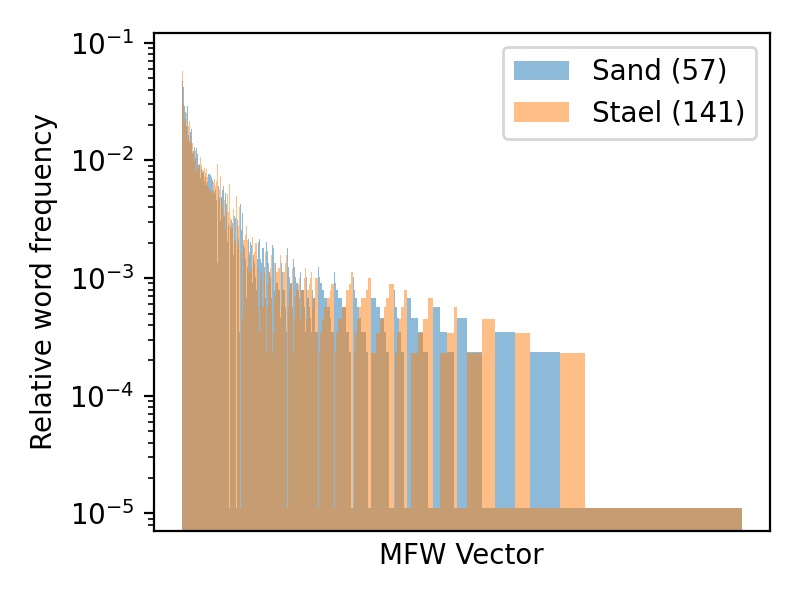
\includegraphics[width=\linewidth]{img/mfw_vector_error_0.png}

  \subcaption{Second example}
  \label{fig:mfw_vector_error_1}
  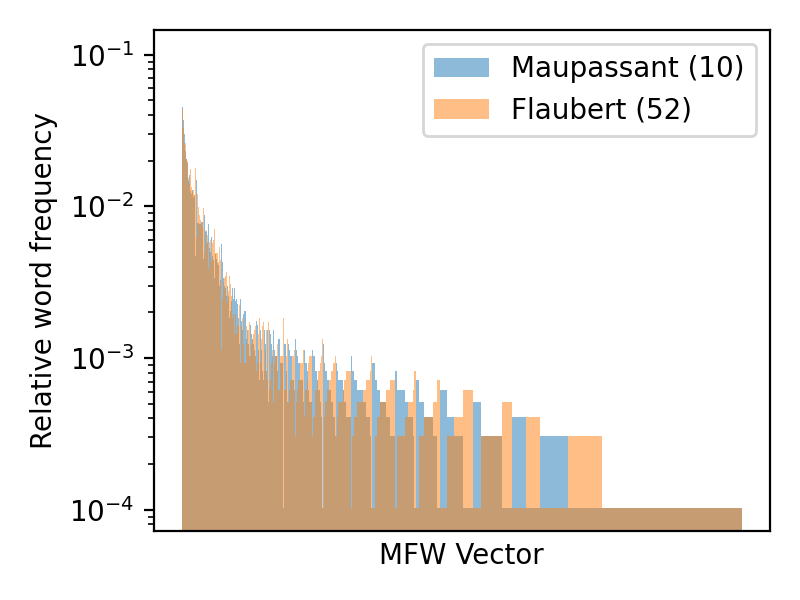
\includegraphics[width=\linewidth]{img/mfw_vector_error_1.png}
\end{figure}

Both document style are close when their feature vector are closely related.
Visually when most the surface overlap, the distance function will give a low value, and rank this link high in the list.
When two vectors are relatively close together determinating that two texts are from a different author can not clearly be established using only one type of representation, no matter the distance metric applied.
The frequent errors vector pairs presented in Figure~\ref{fig:mfw_vector_error} can be visually compared actual true links and actual false links, to have a better understanding of this problematic.
For example the most similar true link (ranked 1 using Manhattan distance) in Figure~\ref{fig:mfw_vector_first_rl} (document 157 from Stael / document 183 from Steal) or the HPrec-th (last continous correct pair from the top of the list) in Figure~\ref{fig:mfw_vector_first_last_rl} (document 107 from France / document 125 from France), both of these links show a large proportion of overlapping surface, like for the frequent errors vectors.
A counter example would be the least similar false link (ranked last using Manhattan distance) which represent a negatively correlated document pair, Figure~\ref{fig:mfw_vector_last_rl} showcase this link (document 136 from Sue / document 188 from Regnier).
As expected, most of this figure surface is non-overlapping.

\begin{figure}
  \centering
  \caption{750-MFW relative frequency for the two documents ranked $X$ in the rank list using Manhattan distance}

  \subcaption{$X$ = First}
  \label{fig:mfw_vector_first_rl}
  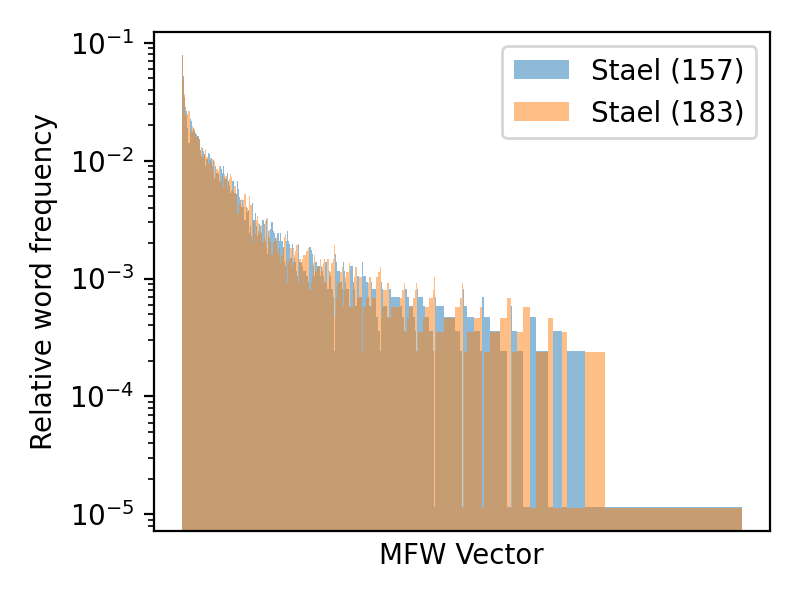
\includegraphics[width=\linewidth]{img/mfw_vector_first_rl.png}

  \subcaption{$X$ = HPrec-th}
  \label{fig:mfw_vector_first_last_rl}
  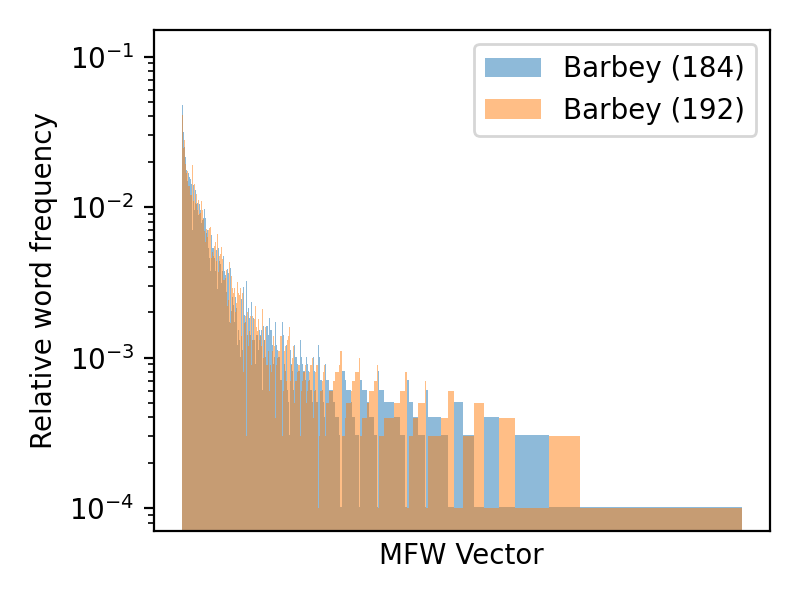
\includegraphics[width=\linewidth]{img/mfw_vector_first_last_rl.png}

  \subcaption{$X$ = Last}
  \label{fig:mfw_vector_last_rl}
  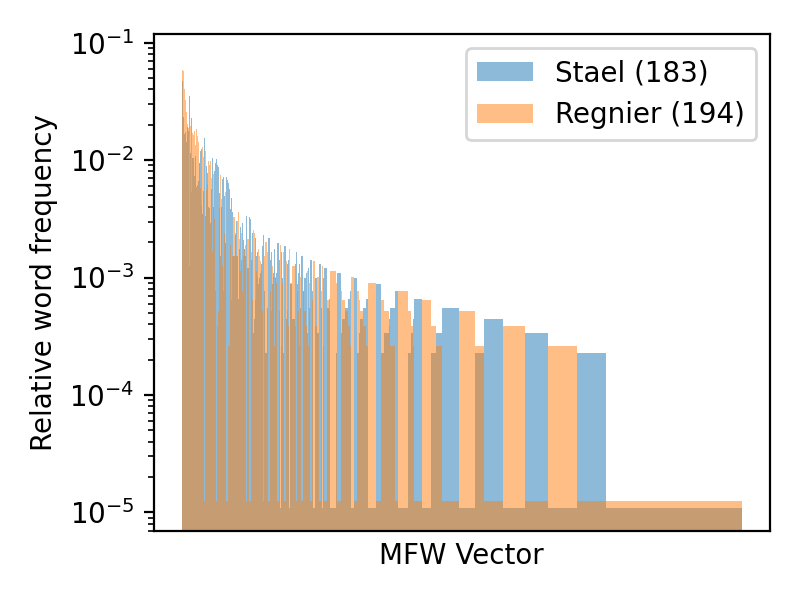
\includegraphics[width=\linewidth]{img/mfw_vector_last_rl.png}
\end{figure}

\subsubsection{Publication date differences analyis}

When dealing with false links ranked high in the rank list, as the previous experiment showed, some excerpt use similar words.
These shared words might be related to the era the book was written in.
The following experiment try to investigate on this.

In the St-Jean dataset publication paper, the publication dates of each excepts are available~\cite{st_jean}.
First the publication date distribution of the dataset must be understood.
Figure~\ref{fig:dates_distribution} show the distribution of the publication date in the St-Jean dataset.
The date difference distribution for each pair of documents can be computed, Figure~\ref{fig:dates_differences_all} showcase this.
The average date difference in the dataset is 28.24 years with a standard deviation of 20.73 years.
Since this dataset contain multiple excerpt from the same book, considering only the links of different authors (false links) is preferable.
Figure~\ref{fig:dates_differences_false} shows the date difference distribution of the false links.
As expected the mean increased from 28.24 years to 29.04 years since there are fewer links with small date difference.
Same authors links (true links) are displayed in Figure~\ref{fig:dates_differences_r_true}, they confirm the previous statement that most of the same authors links have a low date difference with a mean of 5.11 years.

\begin{figure}
  \centering
  \caption{Dates and Date differences denstiy distributions on St-Jean for every excerpt}

  \subcaption{Date distribution}
  \label{fig:dates_distribution}
  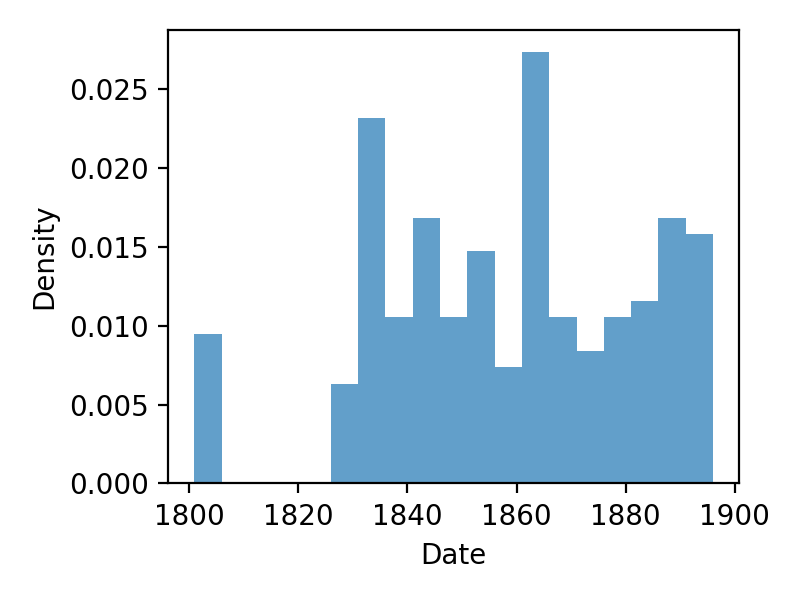
\includegraphics[width=\linewidth]{img/dates_distribution.png}

  \subcaption{Date difference denstiy distributions}
  \label{fig:dates_differences_all}
  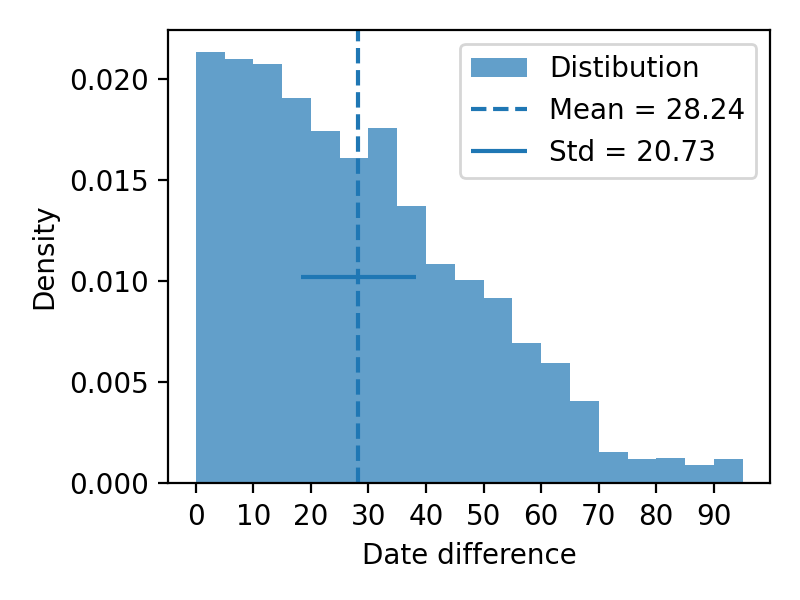
\includegraphics[width=\linewidth]{img/dates_differences_all.png}
\end{figure}

\begin{figure}
  \centering
  \caption{Date difference denstiy distributions in St-Jean}

  \subcaption{False links}
  \label{fig:dates_differences_false}
  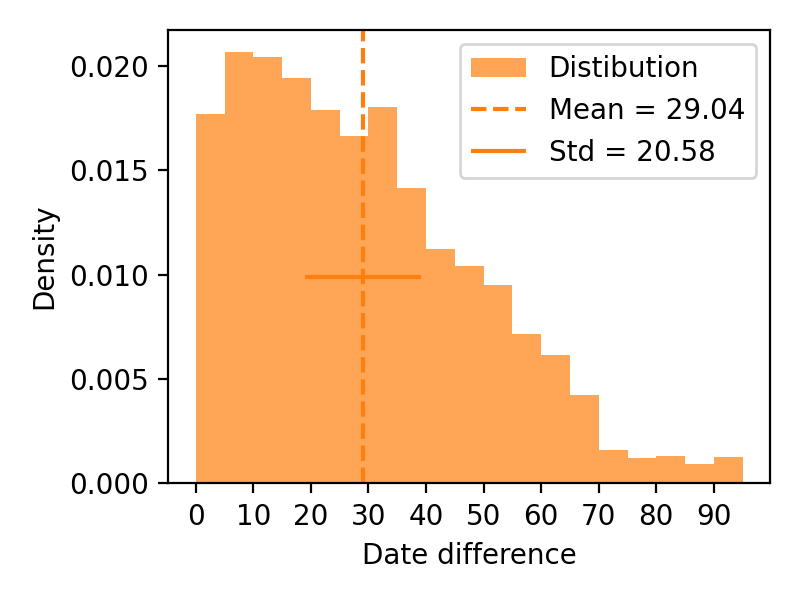
\includegraphics[width=\linewidth]{img/dates_differences_false.png}

  \subcaption{True links}
  \label{fig:dates_differences_r_true}
  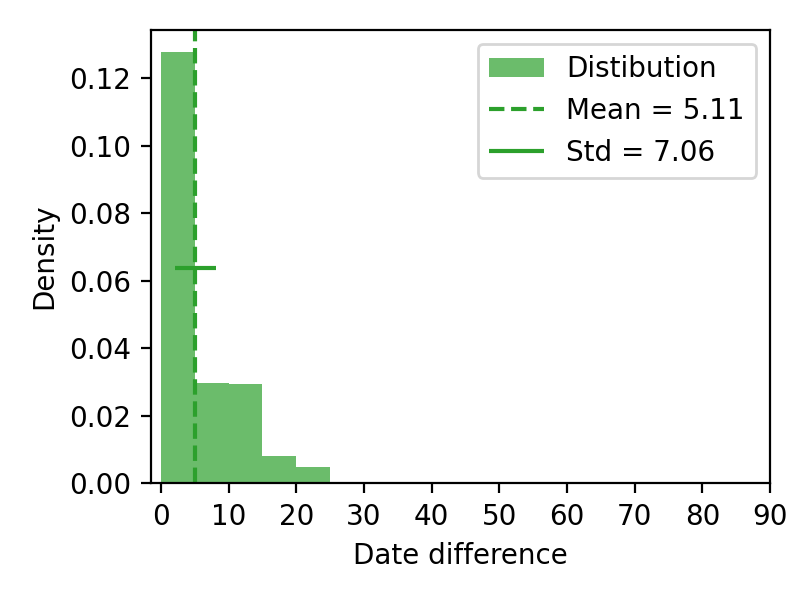
\includegraphics[width=\linewidth]{img/dates_differences_r_true.png}

  \subcaption{Top-r false links using a rank list with 80\% average precision.}
  \label{fig:dates_differences_r_false}
  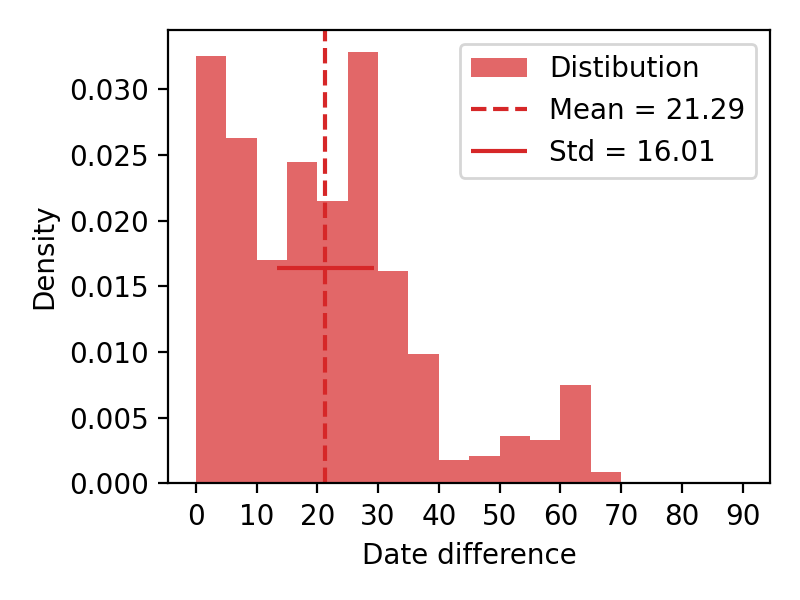
\includegraphics[width=\linewidth]{img/dates_differences_r_false.png}
\end{figure}

The previous statistics can be compared to Figure~\ref{fig:dates_differences_r_false} which show the date difference density on the top-r false links (670 in case of St-Jean) on a rank list with 82\% average precision (obtained by fusing the 4 ranks list used, ref. Section~\ref{sec:rank_list_fusion}~and~\ref{sec:frequent_errors}).
Two interesting information can be extracted here.
First the mean is lower by 7.6 years (29.04 - 21.44) compared to the false links and have a narrow standard deviation distribution which clearly indicate the importance of publication date in the ranking of the documents.
Secondly we can observe a drop after 35 years of date difference, which indicate that links in the interval $\left[0-35\right]$ years are harder to discriminate between a true link and a false link than links outside this interval.
This 35 years interval can be related to the generation factor, the age of woman giving birth is around 25-34 in France~\cite{generations}, the birth country of the authors in this dataset.
Each new generation tend to use its own vocabulary, and thus it can be harder to discriminate the author of text belonging to the same generation, if we assume that the authors write their books at around the same age.
In the other hand having different vocabulary can indicate a different time period and is often used to detect document forgery~\cite{savoy_stylo}.

\subsubsection{Rank lists fusion evaluation}

In this experiment, the goal to understand if fusing rank list can improve performance of the rank list.
The methodology used, is to create $n$ rank lists and fuse them for every $r$ rank lists combinations ($C^n_r$) for the two fusing methods proposed, z-score fusion and regression fusion.

The rank list used are the ones obtained by using the 9 retained rank list methods ($n=9$), see Table~\ref{tab:9rl} in annex.
They represent the best configuration retained for each text representation.
The $r$ value is selected to $4$, since it represents the number of different text representation.
The number of possible fusion combinations is with $n=9$ and $r=4$ is $C^{9}_{4} = 126$.
For this 126 fusions, the 3 metrics: Average Precision (AP), R-Precision (RPrec) and High Precision (HPrec) are computed.

To compare the rank list produced by both the Z-Score fusions and the Regression fusion to the non-fused rank lists, two strategies are used.
One called \textit{Single-Max} which represent the best metrics for each rank list in the fusion and another one called \textit{Single-Mean} which is represented by the mean of each rank list metrics in the fusion.
For example, if for a fusion the average precision of the 4 rank lists are : $0.5, 0.6, 0.7, 0.8$. Single-mean would have an average precision of $0.65$ and Single-max an average precision of $0.8$.

The results of every fusion combinations using the proposed rank list and strategies are graphically presented in Figure~\ref{fig:fusions}.
Statistiques for each metrics and fusion schemes are resumed Tables~\ref{tab:fusion_stats_A_B}/\ref{tab:fusion_stats_B_A}, it contains for each metric, the minimal value (min), the average and the standard deviation (Avg$\pm$Std), the maximal value, the argmin and argmax for the metrics (ids of the rank list presented above).
A sign test between the two strategies and the two fusion methods is presented in Table~\ref{tab:fusion_sign_test}.

\begin{figure}
  \centering
  \caption{Evaluation of every combination of 4 rank list fusions using Z-Score and Regression}
  \label{fig:fusions}

  \subcaption{Testing on St-Jean A (training St-Jean B)}
  \label{fig:fusion_B_A}
  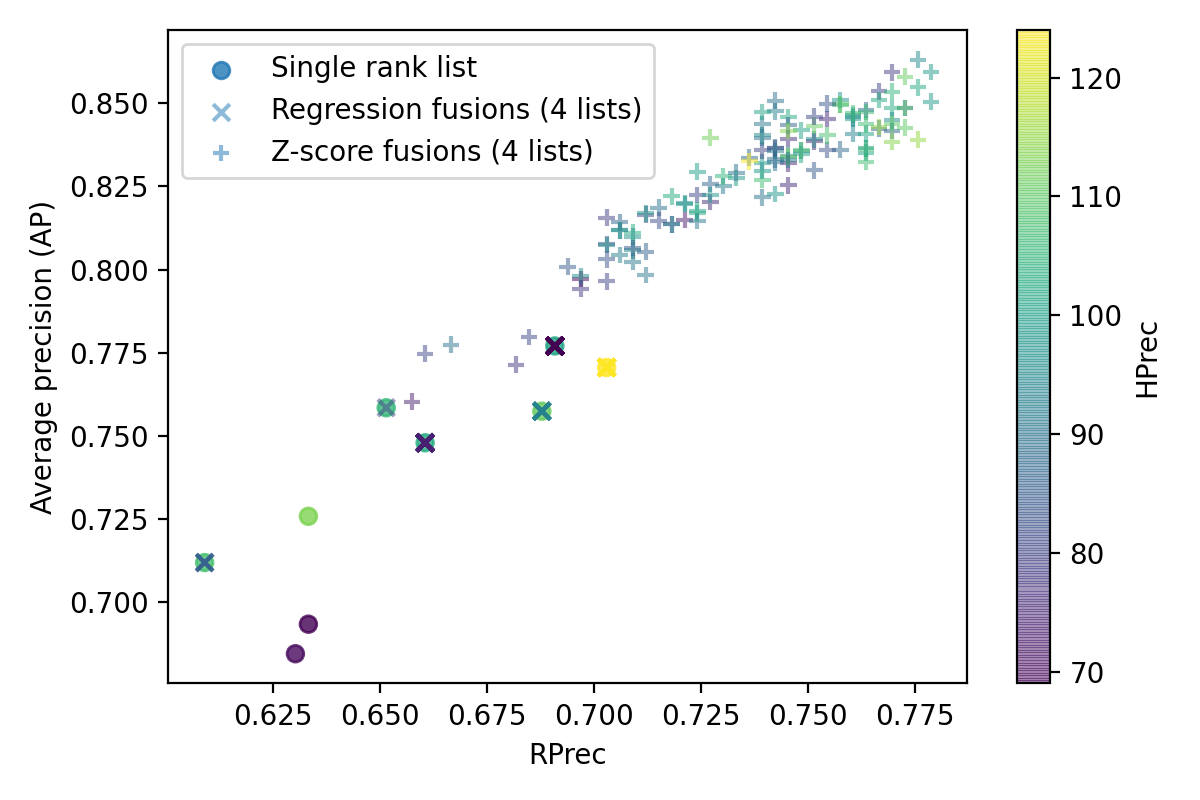
\includegraphics[width=\linewidth]{img/fusion_B_A.png}

  \subcaption{Testing on St-Jean B (training St-Jean A)}
  \label{fig:fusion_A_B}
  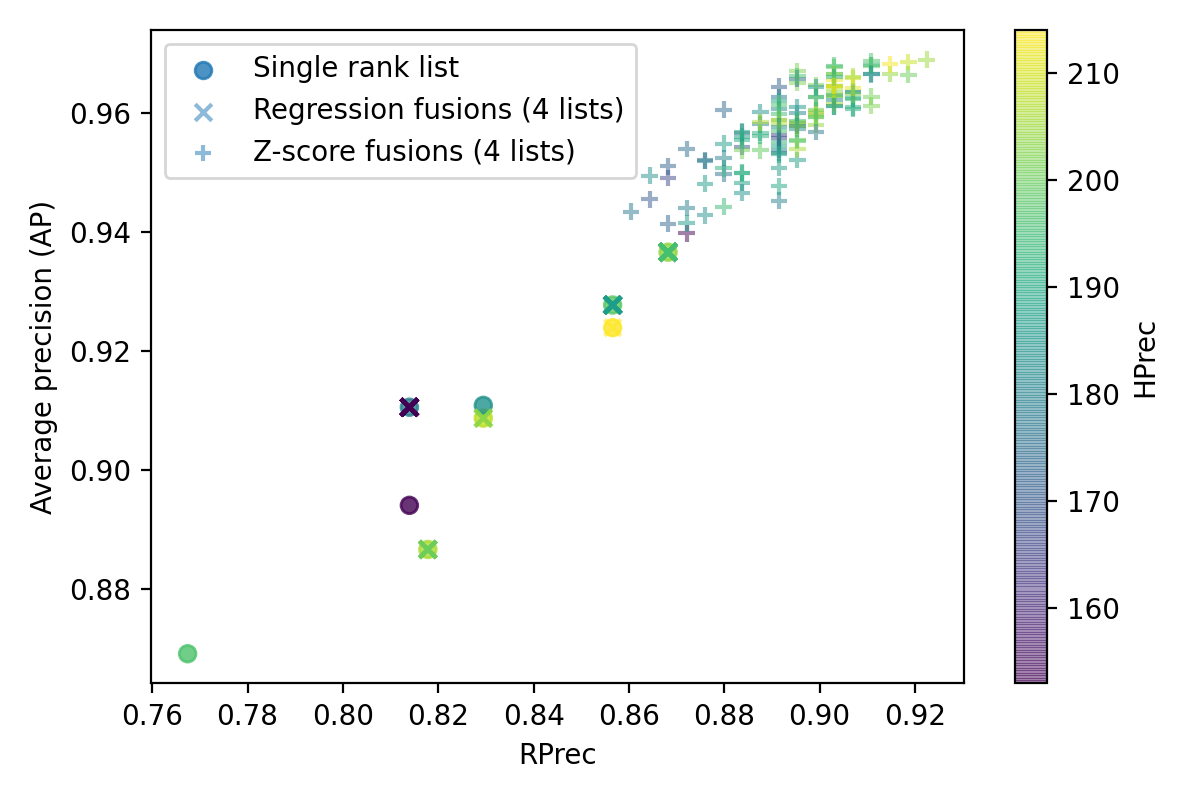
\includegraphics[width=\linewidth]{img/fusion_A_B.png}
\end{figure}

\begin{table}
  \centering
  \caption{Fusion statistics on St-Jean A (training St-Jean B)}
  \label{tab:fusion_stats_A_B}

  \subcaption{Single-Mean}
  \begin{tabular}{l l l l}
    \toprule
    Stats
    & AP
    & RPrec
    & HPrec \\
    \midrule
    Min & $0.704$ & $0.627$ & $42.75$ \\
    Avg$\pm$Std & $0.736\pm0.013$ & $0.656\pm0.012$ & $64.444\pm10.286$ \\
    Max & $0.766$ & $0.686$ & $84.25$ \\
    Argmin & [4,6,7,8] & [4,6,7,8] & [0,1,6,7] \\
    Argmax & [0,2,3,5] & [0,1,2,3] & [2,3,4,8] \\
    \bottomrule
  \end{tabular}

  \subcaption{Single-Max}
  \begin{tabular}{l l l l}
    \toprule
    Stats
    & AP
    & RPrec
    & HPrec \\
    \midrule
    Min & $0.726$ & $0.633$ & $68.0$ \\
    Avg$\pm$Std & $0.769\pm0.009$ & $0.692\pm0.015$ & $88.532\pm9.763$ \\
    Max & $0.777$ & $0.703$ & $99.0$ \\
    Argmin & [4,6,7,8] & [4,6,7,8] & [0,1,6,7] \\
    Argmax & [0,1,2,3] & [0,1,2,3] & [0,1,2,3] \\
    \bottomrule
  \end{tabular}

  \subcaption{Z-Score}
  \begin{tabular}{l l l l}
    \toprule
    Stats
    & AP
    & RPrec
    & HPrec \\
    \midrule
    Min & $0.76$ & $0.658$ & $69.0$ \\
    Avg$\pm$Std & $0.829\pm0.02$ & $0.738\pm0.026$ & $93.833\pm11.108$ \\
    Max & $0.863$ & $0.779$ & $124.0$ \\
    Argmin & [4,5,6,7] & [4,5,6,7] & [0,1,4,5] \\
    Argmax & [0,3,7,8] & [0,3,6,8] & [1,3,6,7] \\
    \bottomrule
  \end{tabular}

  \subcaption{Regression}
  \begin{tabular}{l l l l}
    \toprule
    Stats
    & AP
    & RPrec
    & HPrec \\
    \midrule
    Min & $0.712$ & $0.609$ & $65.0$ \\
    Avg$\pm$Std & $0.764\pm0.016$ & $0.681\pm0.02$ & $72.794\pm12.111$ \\
    Max & $0.777$ & $0.703$ & $99.0$ \\
    Argmin & [4,5,6,7] & [4,5,6,7] & [0,1,2,3] \\
    Argmax & [0,1,2,3] & [2,3,4,5] & [2,3,4,5] \\
    \bottomrule
  \end{tabular}
\end{table}

\begin{table}
  \centering
  \caption{Fusion statistics on St-Jean B (training St-Jean A)}
  \label{tab:fusion_stats_B_A}

  \subcaption{Single-Mean}
  \begin{tabular}{l l l l}
    \toprule
    Stats
    & AP
    & RPrec
    & HPrec \\
    \midrule
    Min          & $0.89$         & $0.80$         & $122.25$      \\
    Avg$\pm$Std & $0.90\pm0.008$ & $0.83\pm0.011$ & $148.11\pm11$ \\
    Max          & $0.92$         & $0.85$         & $172$         \\
    Argmin       & [3,4,7,8]   & [1,3,7,8]   & [1,6,7,8]  \\
    Argmax       & [0,2,5,6]   & [0,2,5,6]   & [0,3,4,5]  \\
    \bottomrule
  \end{tabular}

  \subcaption{Single-Max}
  \begin{tabular}{l l l l}
    \toprule
    Stats
    & AP
    & RPrec
    & HPrec \\
    \midrule
    Min          & $0.91$         & $0.82$         & $153.25$      \\
    Avg$\pm$Std & $0.93\pm0.008$ & $0.86\pm0.012$ & $174.8\pm7$ \\
    Max          & $0.93$         & $0.87$         & $182$         \\
    Argmin       & [3,4,7,8]   & [1,3,7,8]   & [1,6,7,8]  \\
    Argmax       & [0,1,2,3]   & [0,1,2,3]   & [0,1,2,5]  \\
    \bottomrule
  \end{tabular}

  \subcaption{Z-Score}
  \begin{tabular}{l l l l}
    \toprule
    Stats
    & AP
    & RPrec
    & HPrec \\
    \midrule
    Min          & $0.94$         & $0.86$         & $153$      \\
    Avg$\pm$Std & $0.96\pm0.006$ & $0.89\pm0.012$ & $191.3\pm12$ \\
    Max          & $0.97$         & $0.82$         & $214$         \\
    Argmin       & [1,2,3,8]   & [2,3,4,8]   & [1,2,3,8]  \\
    Argmax       & [1,2,5,6]   & [1,2,5,6]   & [2,3,5,7]  \\
    \bottomrule
  \end{tabular}

  \subcaption{Regression}
  \begin{tabular}{l l l l}
    \toprule
    Stats
    & AP
    & RPrec
    & HPrec \\
    \midrule
    Min          & $0.88$         & $0.81$         & $124$      \\
    Avg$\pm$Std & $0.92\pm0.015$ & $0.85\pm0.024$ & $152.9\pm18$ \\
    Max          & $0.94$         & $0.87$         & $182$         \\
    Argmin       & [3,4,5,6]   & [1,2,3,4]   & [1,2,3,4]  \\
    Argmax       & [0,1,2,3]   & [0,1,2,3]   & [5,6,7,8]  \\
    \bottomrule
  \end{tabular}
\end{table}

\begin{table*}
  \centering
  \caption{Rank list fusion sign test. \textit{The star (*) indicate a Binomial test p-value smaller than 5\%}}
  \label{tab:fusion_sign_test}

  \subcaption{Testing St-Jean A (training St-Jean B)}
  \label{tab:fusion_A_B}
  \begin{tabular}{l c c c c}
    \toprule
    Metric
    & Z-Score/T/Single-Mean
    & Z-Score/T/Single-Max
    & Regression/T/Single-Mean
    & Regression/T/Single-Max\\
    \midrule
    AP    & *126/0/0 & *126/0/0  & *108/0/18 & 0/81/45* \\
    RPrec & *126/0/0 & *125/1/0  & *92/4/30  & 0/78/48* \\
    HPrec & *126/0/0 & *111/0/14 & *79/1/46  & 0/14/112*\\
    \bottomrule
  \end{tabular}

  \subcaption{Testing St-Jean B (training St-Jean A)}
  \label{tab:fusion_B_A}
  \begin{tabular}{l c c c c}
    \toprule
    Metric
    & Z-Score/T/Single-Mean
    & Z-Score/T/Single-Max
    & Regression/T/Single-Mean
    & Regression/T/Single-Max \\
    \midrule
    AP    & *126/0/0 & *124/0/2 & *120/0/6  & 0/85/41* \\
    RPrec & *126/0/0 & *119/2/5 & *114/0/12 & 0/76/50* \\
    HPrec & *124/0/2 & *73/3/45 & *92/0/34  & 0/25/101*\\
    \bottomrule
  \end{tabular}

\end{table*}

Using these distance metrics on St-jean, the sign test tends to indicate that the fusion increase the overall quality of the rank list.
The three evaluations metrics are high correlated (especially average precision and R-Precision), only the average precision will be explored in depth.
The Z-Score fusion, produce for every metrics better results than both Single-Mean and Single-Max, the average precision is increase in average by \~10\% compared to the average of the average precision (Single-Mean) of the rank list used, and by ~6\% in average when considering the maximal average precision (Single-Max).
In the other hand, the Regression fusion, have an average increase of \~3\% in average precision for the Single-Mean and have a decrease of ~1\% when comparing to the Single-Max.
The results of fusing multiple rank lists when using regression fusion strategy tends to indicate that the resulting rank list in average share the quality of the best rank list used with some slight decreases.
No particular set of rank list tends to give the best results in every case when fusing with the two strategies, every rank list is present in the argmax, but with the Z-Score fusion, the best results seem to be obtained with rank lists using different text representations.
The Z-score fusion give the best results overall.


\newpage
\subsection{Clustering}

\subsubsection{Clustering evaluation metrics}

\begin{definition}[Cluster difference]
  This metric aim to evaluate if the clustering found the right number of cluster.
  The cluster difference is the number cluster found $p$ minus the actual number of cluster $k$.
  \begin{equation}
    Cluster_{diff} = p - k
  \end{equation}
  A positive value indicate an overestimation of the real number of cluster, a negative value indicate the underestimation.
  Zero indicate that the right number of cluster was found.
  This value can be normalized by the number of documents N, which correspond to the difference of the r ratios.
  As stated in the PAN16 evaluation campaign paper, estimating correctly the r ratio tends to indicate a good clustering~\cite{pan16}.
  \begin{equation}
    r_{diff} = \frac{p}{N} - \frac{k}{N} = \frac{p - k}{N}
  \end{equation}
\end{definition}

To evaluate clustering, the metrics used are the BCubed~\cite{bcubed} family.
BCubed has shown to satisfy 4 following importants constraints when evaluating clusterings : \textit{Cluster Homogeneity} (different categories should be in the different clusters), \textit{Cluster Completness} (same categories should belong to the same cluster) and the \textit{Rag Bag constraint} (noisy/miscellaneous categories should be in the same cluster and not in 'healthy' clusters) and the \textit{Cluster size vs quantity constraints} (favorise large cluster)~\cite{bcubed}.
These metrics are used in the clustering task at PAN@CLEF~\cite{pan16}.

\begin{definition}[Correctness~\cite{bcubed}]
  The $BCubed$ metric family is based on the the following \textit{Correctness} principle.
  Let L(e) and C(e) be the category and the cluster of an element e.
  The Correctness is following the biconditional condition on the category and cluster equality (biconditional: $A \Longleftrightarrow B \equiv (A \land B) \lor (\neg A \land \neg B)$).
  \begin{gather*}
    Correctness(e, e') = \\
    \begin{cases}
      1, & if (L(e) = L(e')) \Longleftrightarrow (C(e) = C(e'))\\
      0, & otherwise
    \end{cases}
  \end{gather*}
  In other terms, the correctness has a value of one (100\% correct) if the two elements are in the both in the same cluster and has the same category OR both in a different cluster and a different category.
\end{definition}

\begin{definition}[$BCubed$ Precision~\cite{bcubed}]
  The $BCubed$ Precision correspond to the average of correctness for all elements on the average of all element such that \textbf{their clusters are the same}.
  \begin{equation}
    BCubed_{precision} = \text{Avg}_{e}[\text{Avg}_{e' C(e)=C(e')}[Correctness(e, e')]]
  \end{equation}
\end{definition}

\begin{definition}[$BCubed$ Recall~\cite{bcubed}]
  The $BCubed$ Recall correspond to the average of correctness for all elements on the average of all element such that \textbf{their categories are the same}.
  \begin{equation}
    BCubed_{recall} = \text{Avg}_{e}[\text{Avg}_{e' L(e)=L(e')}[Correctness(e, e')]]
  \end{equation}
\end{definition}

\begin{definition}[$BCubed F_1$ Score~\cite{bcubed}]
  $BCubed F_1$ Score uses the harmonic mean between the $BCubed_{precision}$ and $BCubed_{recall}$.
  \begin{equation}
    BCubed_{F_1} =
    2 \cdot \frac{BCubed_{precision} \cdot BCubed_{recall}}
    {BCubed_{precision} + BCubed_{recall}}
  \end{equation}
  The $F_\beta$ measures, not shown here, provide a parametric way to represent with a single value the two counterbalancing measures in this case, the $BCubed F_1$ is computed using the $F$ measures with $\beta = 1$ and the $BCubed$ Precision and Recall scores.
\end{definition}

\subsubsection{Clustering unsupervised cut method}

For this experiment, the goal is to test the unsupervised cut method based on the IPS (Iterative positive silhouette) Procedure on the literature dataset.
When applying the procedure, the number of clusters start at 2, each iteration the silhouette score is computed if it reaches a negative value the procedure stop otherwise the number of cluster is increased and the process is repeated.

The rank list used for this experiment is the one generated using Z-score fusion with retained text representation (9 for St-Jean and 7 for Brunet and Oxquarry), see Section~\ref{sec:annex_retained_text_representation} in annex.

When running the IPS procedure on the dataset, on Figures~\ref{fig:unsupervised_clustering} the silhouette score is indicated as each step and compared to the three BCubed metrics.
For the sake of the experiment, the agglomerative clustering is also run up to a number of cluster equal to the number of documents (singleton clusters).
Since the rank list used for the clustering is not perfect (every true links at the top), there is no number of cluster with a BCubed $F_1$ score of 1.0.
The estimated number of cluster is on every dataset overestimated, average r-ratio difference of $0.21$, which means that the median neareast-cluster distance is greater than the median intra-cluster distance even when dealing with the right number of clusters.
This can be due to the fact that the rank list is not perfect.
To mitigate this problem, an easy solution would be to the stop the procedure at for example : $0.1$ instead of $0$.

\begin{table*}
  \centering
  \caption{Unsupervised clustering evaluation on the datasets}
  \label{tab:unsupervised_clustering}
    \begin{tabular}{l c c c c}
      \toprule
      &
      BCubed $F_1$ Score &
      BCubed Precision &
      BCubed Recall &
      r ratio differences \\
      \midrule
      Oxquarry         & 0.73 & 1.00 & 0.58 & 0.23\\
      Brunet           & 0.82 & 0.94 & 0.72 & 0.11\\
      St-Jean A        & 0.66 & 1.00 & 0.49 & 0.22\\
      St-Jean B        & 0.73 & 1.00 & 0.58 & 0.27\\
      \textbf{Average} &
      \textbf{0.74} &
      \textbf{0.98} &
      \textbf{0.59} &
      \textbf{0.21} \\
      \bottomrule
    \end{tabular}
\end{table*}

\begin{figure}
  \caption{Unsupervised clustering example on Brunet and St-Jean B}
  \label{fig:unsupervised_clustering}

  \subcaption{Brunet}
  \label{fig:unsupervised_clustering_brunet}
  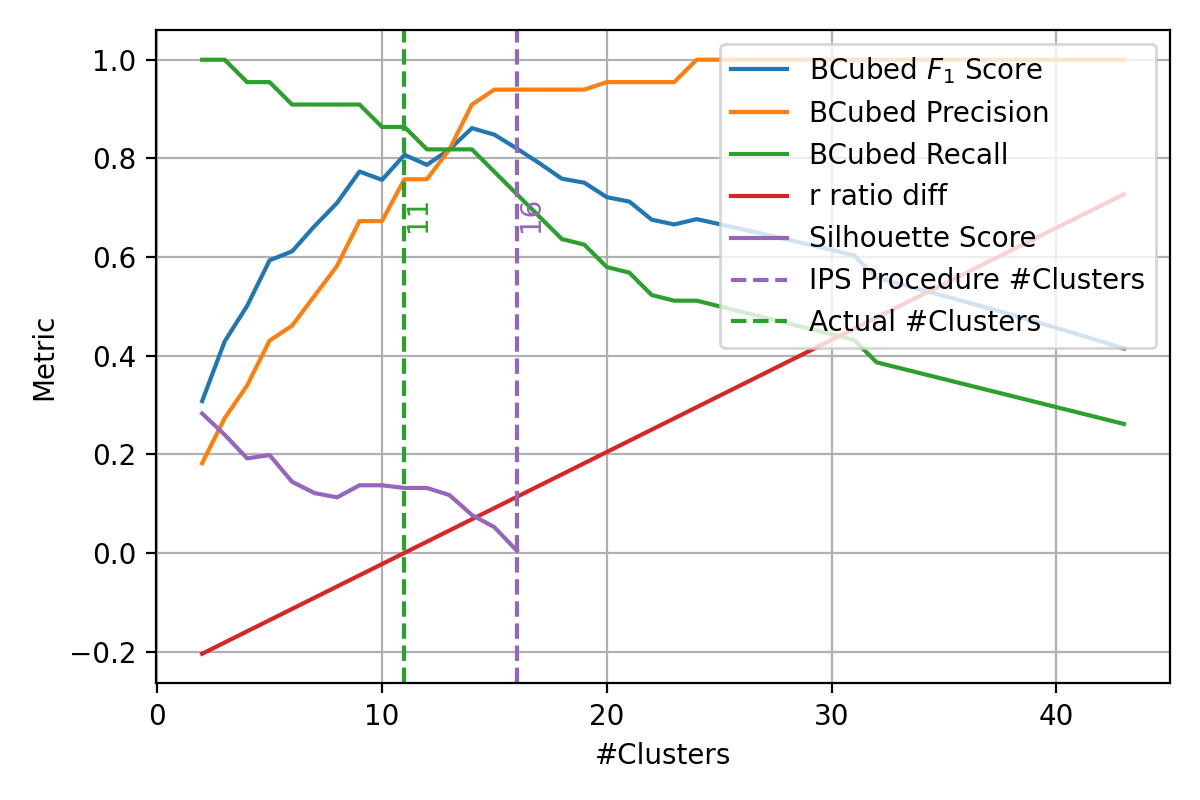
\includegraphics[width=\linewidth]{img/unsupervised_clustering_brunet.png}

  \subcaption{St-Jean B}
  \label{fig:unsupervised_clustering_st_jean_B}
  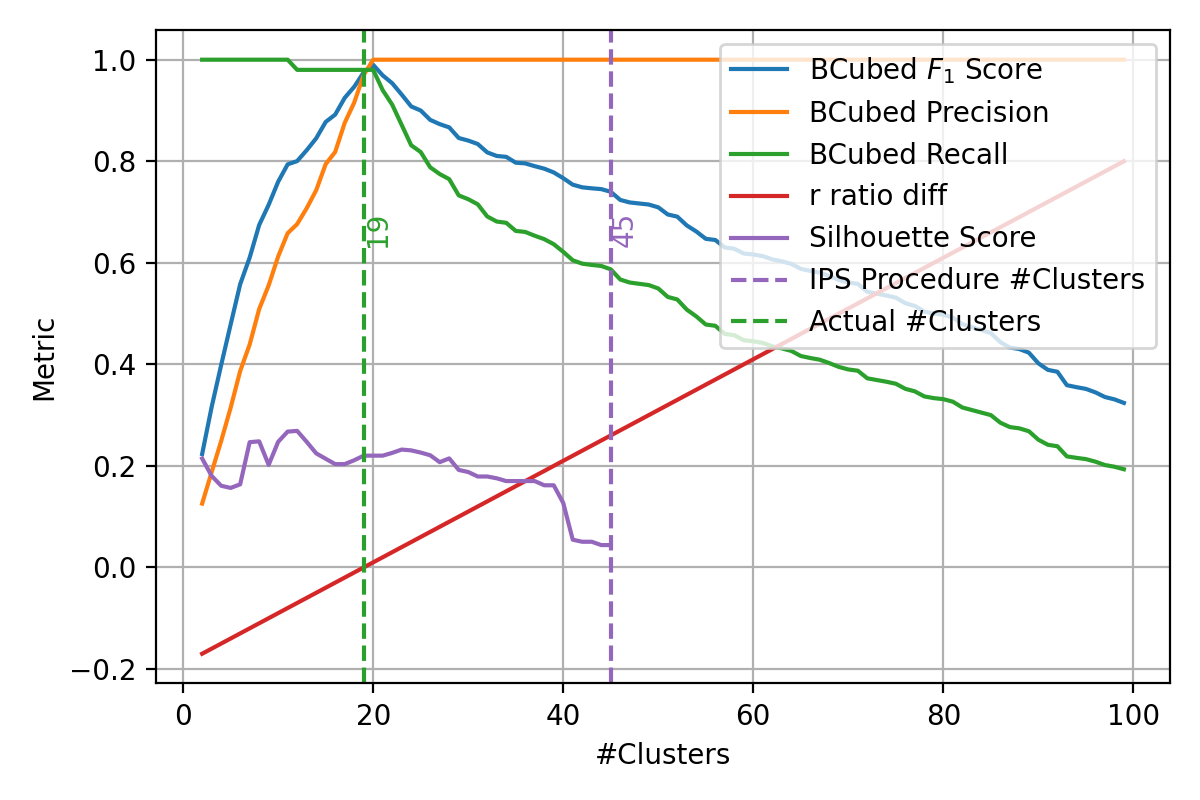
\includegraphics[width=\linewidth]{img/unsupervised_clustering_st_jean_B.png}
\end{figure}

\subsubsection{Clustering with the supervised cut method}

To evaluate the supervised clustering approach, every dataset were used.
First a rank list for each dataset is computed using a z-score fusion using the retained rank list, see Section~\ref{sec:annex_retained_text_representation} in annex.
Then every pair of rank list is used to create a training/testing evaluation.
In other words, a model to create cuts is trained on every dataset and tested on all the datasets.

The model does not depend on the rank list size since only relative magnitudes are used.
An example of a run using the St-Jean A as training set and St-Jean B as testing is shown visually in Figure~\ref{fig:supervised_clustering_sj}.
The BCubed $F_1$ scores computed during this experiment are in Table~\ref{tab:training_testing_f_1} and the r ratio difference
in Table~\ref{tab:training_testing_r_diff}

Multiple points can be observed with these results:
\begin{itemize}
  \item
  When testing the cut model, having a rank list of good quality tends to produce better clustering, no matter the quality of the rank list used for the training.
  \item
  Using the best rank list for training the cut model does not always give the best results.
  An example to illustrate this observation, the St-Jean B dataset have the best rank list (0.93 AP) when using a model trained on this rank list, it produces a cut with the following F1 scores : 0.78/0.74/0.81/0.93.
  In the other hand, when using Oxquarry for the training with a rank list of 0.72 AP, the F1 score obtained are : 0.82/0.82/0.86/0.95, which is clearly better results.
  \item
  The statement made during the PAN16 campaign claiming that finding the right number of cluster give a better clustering can be observed by comparing the BCubed $F_1$ scores in Table~\ref{tab:training_testing_f_1} to the r ratios differences in Figure~\ref{tab:training_testing_r_diff}.
  When a low r-ratio difference occure, the results tends to show that a large B-Cubed $F_1$ score is obtained, and vice versa.
\end{itemize}

\begin{figure}
  \caption{Supervised clustering example}
  \label{fig:supervised_clustering_sj}

  \subcaption{Testing on St-Jean A (training St-Jean A)}
  \label{fig:supervised_clustering_testing_st_jean_A_with_st_jean_A}
  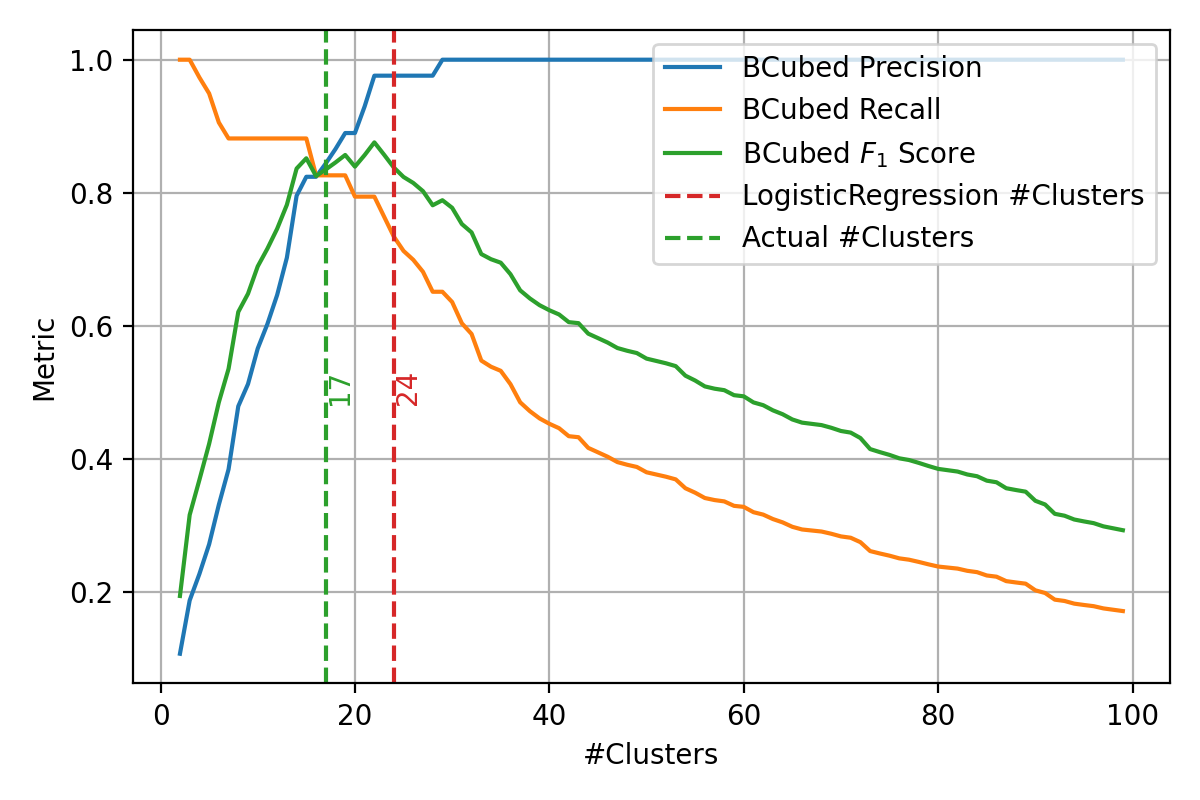
\includegraphics[width=\linewidth]{img/supervised_clustering_testing_st_jean_A_with_st_jean_A.png}

  \subcaption{Testing on St-Jean B (training on St-Jean A)}
  \label{fig:supervised_clustering_testing_st_jean_B_with_st_jean_A}
  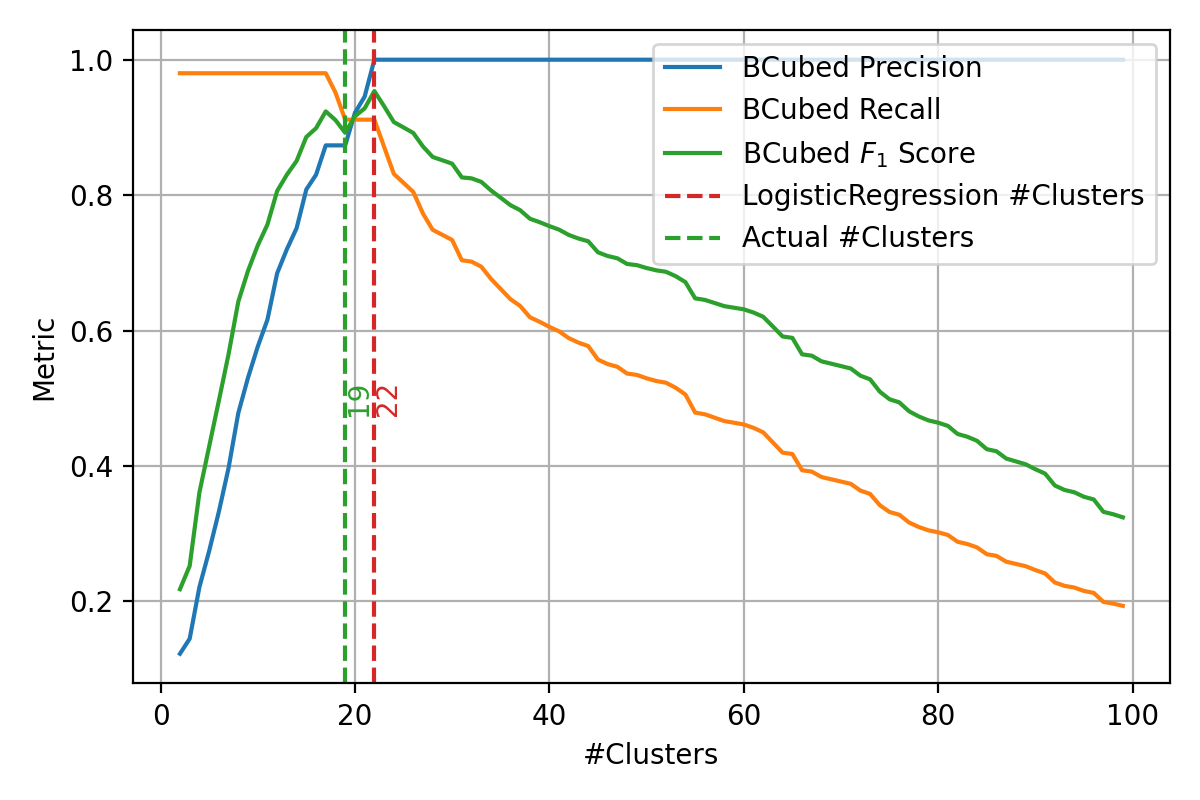
\includegraphics[width=\linewidth]{img/supervised_clustering_testing_st_jean_B_with_st_jean_A.png}
\end{figure}

\begin{table*}
  \centering
  \caption{Supervised clustering evaluation}
  \label{tab:supervised_clustering}

  \subcaption{Every possible training testing dataset pairs. Metrics in order : BCubed $F_1$ Score / BCubed Precision / BCubed Recall / r ratio difference}
  \label{tab:supervised_clustering_train_test}
  \begin{tabular}{l l| c c c c}
    \toprule
    \multicolumn{2}{c}{\multirow{2}{*}{}} & \multicolumn{4}{c}{Testing}\\
    \multicolumn{2}{c}{}
                    & Oxquarry & Brunet & St-Jean A & St-Jean B \\
        \midrule
    \parbox[t]{2mm}{\multirow{4}{*}{\rotatebox[origin=c]{90}{Training}}}
        & Oxquarry
        & 0.82/1.00/0.70/0.08
        & 0.86/0.91/0.82/0.07
        & 0.91/0.87/0.95/-0.03
        & 0.92/0.88/0.98/-0.02
        \\
        & Brunet
        & 0.80/1.00/0.67/0.10
        & 0.75/0.94/0.62/0.18
        & 0.79/0.96/0.67/0.09
        & 0.92/1.00/0.86/0.04
        \\
        & St-Jean A
        & 0.80/1.00/0.67/0.10
        & 0.82/0.94/0.73/0.11
        & 0.87/0.93/0.81/0.03
        & 0.93/0.93/0.94/0.00
        \\
        & St-Jean B
        & 0.80/1.00/0.67/0.10
        & 0.76/0.94/0.64/0.16
        & 0.81/0.96/0.70/0.08
        & 0.92/1.00/0.86/0.04
        \\
        \bottomrule
  \end{tabular}

  \subcaption{Metrics averages}
  \label{tab:supervised_clustering_average}
  \begin{tabular}{l c c c c}
    \toprule
    &
    BCubed $F_1$ Score &
    BCubed Precision &
    BCubed Recall &
    r ratio differences \\
    \midrule
    \textbf{Average}
    & \textbf{0.84}
    & \textbf{0.95}
    & \textbf{0.77}
    & \textbf{0.07}
    \\
    \bottomrule
  \end{tabular}
\end{table*}
